\chapter{Diseño}

En el presente capítulo, se ofrece una descripción detallada de las clases que constituyen los diversos subsistemas, las bases de datos que almacenan la información crítica y los servidores que sustentan la operatividad del sistema. Se presentan, además, los diagramas de clases específicos para cada uno de estos subsistemas, proporcionando una visión clara de su estructura interna y las relaciones entre sus entidades. Adicionalmente, se incluyen diagramas de componentes que desglosan la arquitectura de las pantallas que conforman la aplicación móvil, ilustrando su organización y dependencias. Finalmente, se exploran los diagramas de secuencia, los cuales representan de manera exhaustiva las dinámicas trayectorias de interacción definidas por los casos de uso del sistema.

\section{Diagrama de la Estructura General del Sistema} 
La Figura \ref{fig:Diagrama de sistemas} ilustra la arquitectura general del sistema propuesto, presentando los principales componentes que lo integran y sus interconexiones. 

En este diagrama de alto nivel, se distinguen tres capas fundamentales: la capa de datos, la capa de servicios y la capa de presentación. 

La capa de datos está representada por una base de datos PostgreSQL alojada en la plataforma Railway. Esta base de datos se comunica de manera segura mediante el protocolo SSL con el Servidor Java Spring-Boot, el cual reside en la plataforma Azure. 

La capa de servicios se compone de dos servidores principales, ambos desplegados en Azure. El primero es el Servidor Java Spring-Boot, que actúa como el núcleo de la lógica de negocio y gestiona el acceso a la base de datos. El segundo es el Servidor Red Neuronal, encargado de las funcionalidades específicas relacionadas con redes neuronales y el reconocimiento facial. 


La capa de presentación se compone de dos clientes principales: el Sistema Web (Simulación SAES y DAE), desplegado localmente, y la App Móvil. Ambos clientes se comunican con los servidores en Azure mediante el protocolo HTTPS, garantizando una comunicación segura, también, el Sistema Web interactúa directamente con el Servidor Java Spring-Boot, mientras que la App Móvil se comunica tanto con el Servidor Java Spring-Boot como con el Servidor Red Neuronal, también a través de HTTPS.

\begin{figure}[htbp!]
	\begin{center}
		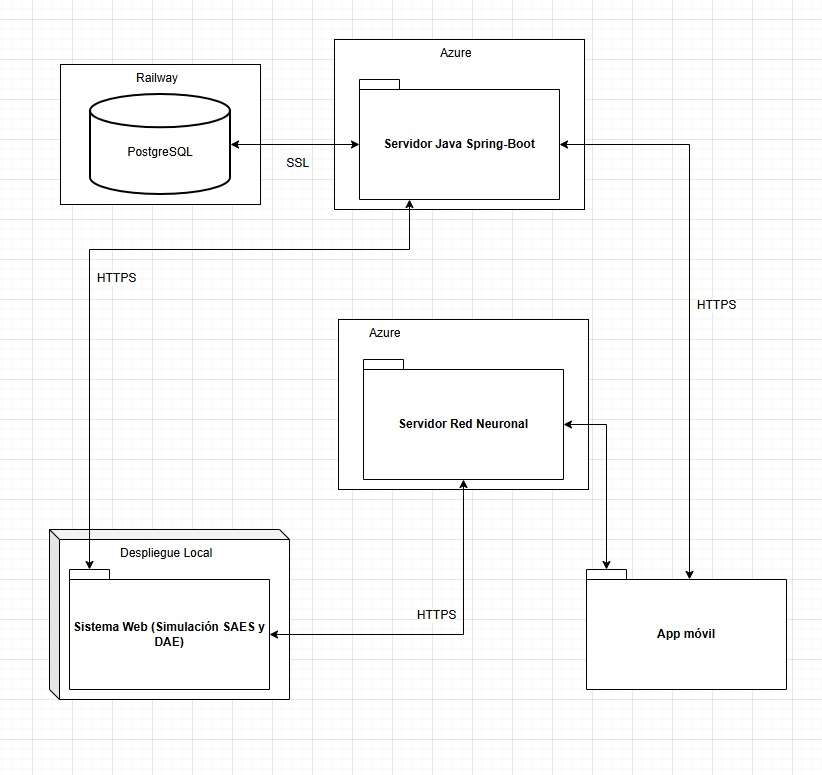
\includegraphics[width=0.8\textwidth]{images/DiagramaGeneralClases}
		\caption{Diagrama de la Estructura General del Sistema.}
		\label{fig:Diagrama de sistemas}
	\end{center}
\end{figure}

A continuación se entrara más en detalle en la estructura interna de los componentes del sistema del diagrama anterior.

\newpage

\section{Estructura Interna Detallada de la Aplicación Móvil} 

La Figura \ref{fig:Diagrama_app_movil_detallado} profundiza en la arquitectura interna de la aplicación móvil, presentando los paquetes y componentes clave que la conforman. 

El punto de entrada principal de la aplicación es la actividad `MainActivity.kt`, la cual orquesta el flujo general de la aplicación. 

La interfaz de usuario de la aplicación se construye dentro del paquete `Pantallas`. Este paquete contiene las implementaciones de las pantallas de la aplicación utilizando Jetpack Compose. Cada pantalla se define mediante funciones Composable, que describen la estructura y el comportamiento de la interfaz de usuario de manera declarativa. 

La lógica de presentación y la gestión del estado de las `Pantallas` se encuentran en el paquete llamado `com.example.prueba3.Views`. Dentro de este paquete, los ViewModels actúan como intermediarios, proporcionando los datos necesarios a las Composables y manejando la lógica de las interacciones del usuario. Existe una relación directa entre las `Pantallas` y los `Views`, donde cada pantalla suele estar asociada a un ViewModel específico. 

El modelo de datos de la aplicación se define principalmente en el paquete `com.example.prueba3.Clases`. Este paquete contiene las clases que representan los datos utilizados por la aplicación. En su mayoría, estas clases son Data Classes, diseñadas para almacenar y transportar datos de manera concisa y eficiente.

La comunicación con los servicios backend se gestiona a través del paquete `RetroFit`. Este paquete contiene las interfaces de Retrofit que definen los endpoints de la API de los servidores remotos. Estas interfaces especifican las operaciones HTTP (GET, POST y DELETE) necesarias para interactuar con el Servidor Java Spring-Boot y el Servidor Red Neuronal. Retrofit se encarga de generar el código necesario para realizar estas solicitudes y procesar las respuestas del servidor.

\newpage

\begin{figure}[htbp!]
	\begin{center}
		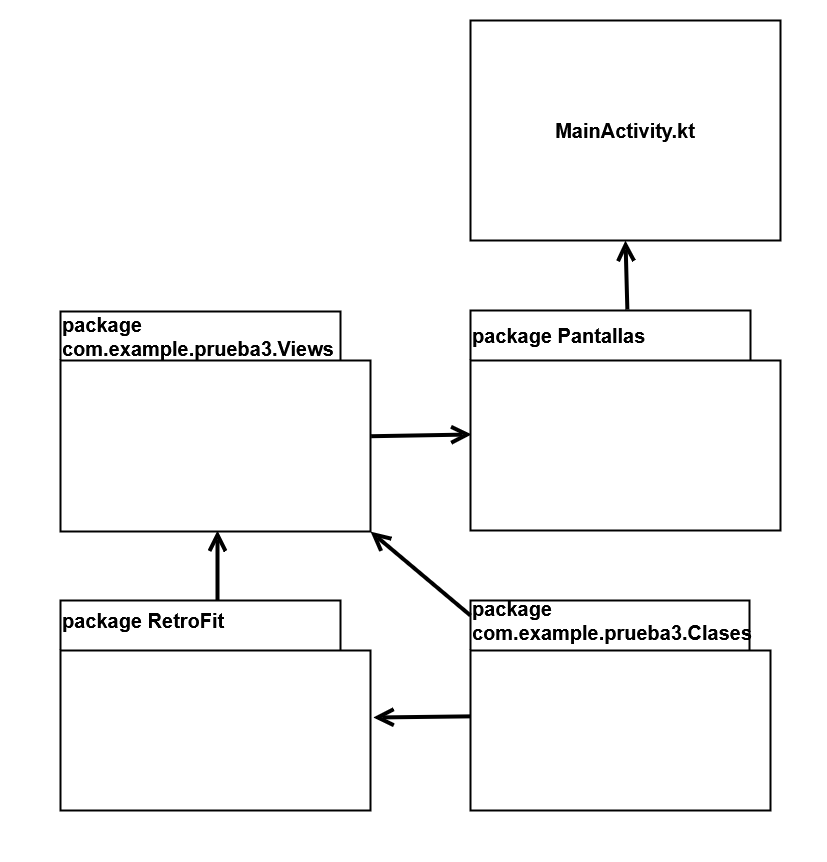
\includegraphics[width=0.6\textwidth]{DiagramasMoviles/DCM (1)}
		\caption{Estructura Interna Detallada de la Aplicación Móvil por Paquetes.}
		\label{fig:Diagrama_app_movil_detallado}
	\end{center}
\end{figure}



A continuación, se presentarán las clases contenidas en los paquetes `com.example.prueba3.Views` (ViewModels), `com.example.prueba3.Clases` (Data Classes) y las interfaces definidas en el paquete `RetroFit`, detallando su estructura y funcionalidad sección por sección. Adicionalmente, se incluirán diagramas de componentes específicos para cada una de las `Pantallas` de la aplicación móvil, ilustrando la composición de sus elementos y sus dependencias internas.

\newpage

\subsection{Diagramas de Componentes de Pantallas}

Para una comprensión más profunda de la arquitectura de la interfaz de usuario de la aplicación móvil, a continuación se presentan los diagramas de componentes para cada una de las pantallas principales. Estos diagramas ilustran la composición interna de cada pantalla, mostrando los elementos de la interfaz de usuario (Composables), los datos que manejan y las posibles interacciones o dependencias con otros componentes. Cada diagrama proporciona una vista modular de la pantalla, facilitando la visualización de cómo se construyen las distintas secciones de la interfaz de usuario y cómo se relacionan entre sí. La Figura \ref{fig:Pantallas} muestra las pantallas (archivos .kt) presentes en package.Pantallas.

\begin{figure}[htbp!]
	\begin{center}
		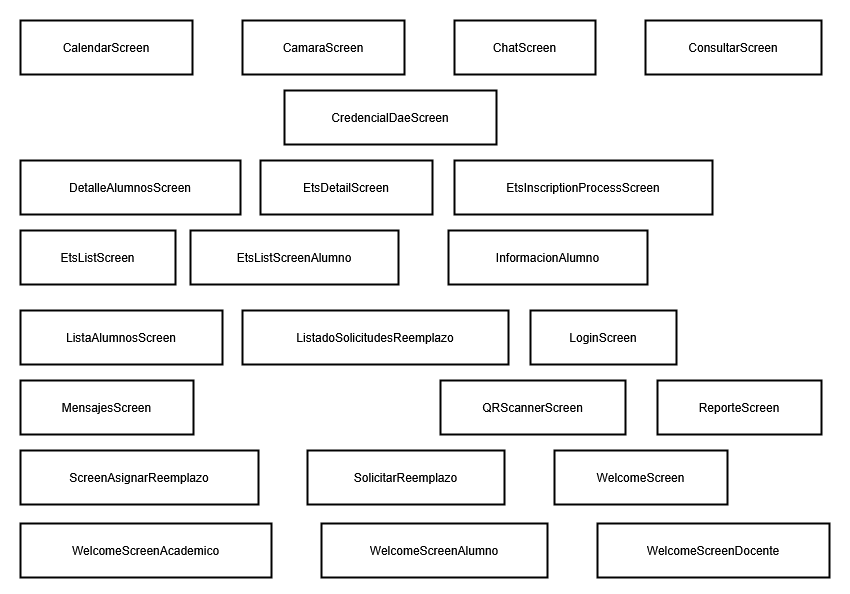
\includegraphics[width=0.9\textwidth]{DiagramasMoviles/DCM (12)}
		\caption{Pantallas presentes en package.Pantallas (archivos .kt).}
		\label{fig:Pantallas}
	\end{center}
\end{figure}


\newpage

\subsection{Diagrama de Componentes de CalendarScreen.kt}

La Figura \ref{fig:Componentes_1} muestra el diagrama de componentes para CalendarScreen.kt que es un composable que contiene a la \IUref{IU02}{Pantalla Consultar calendario escolar}, que muestra el calendario escolar y permite al usuario ver cuantos días faltan para el periodo de ETS próximo si esta disponible.

\begin{figure}[htbp!]
	\begin{center}
		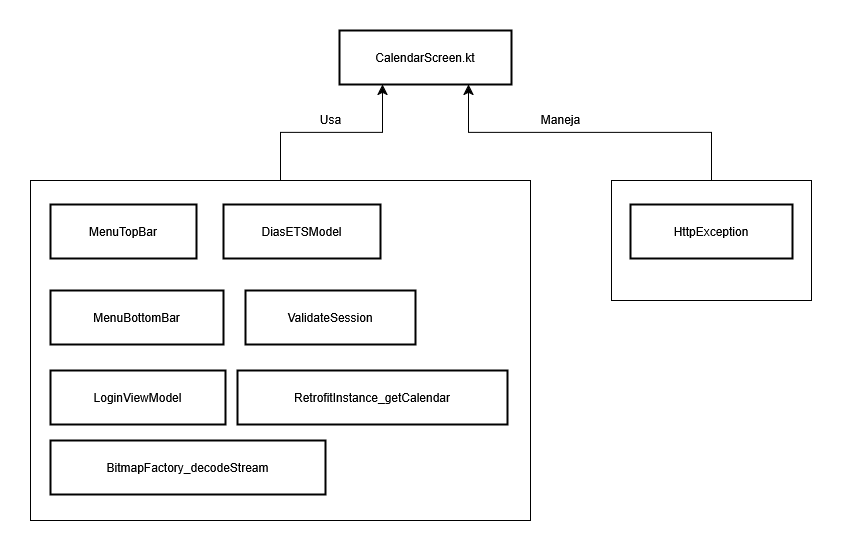
\includegraphics[width=0.9\textwidth]{DiagramasMoviles/DCM (13)}
		\caption{Diagrama de componentes para CalendarScreen.kt .}
		\label{fig:Componentes_1}
	\end{center}
\end{figure}

\newpage

\subsection{Diagrama de Componentes de CamaraScreen.kt}

La Figura \ref{fig:Componentes_2} muestra el diagrama de componentes para CamaraScreen.kt que es un composable que contiene a la \IUref{IU17}{Pantalla de Reconocimiento facial} y la \IUref{IU19}{Pantalla de Reconocimiento facial alumno}, que muestran la cámara usada para obtener la foto que se usara para el proceso de reconocimiento facial.

\begin{figure}[htbp!]
	\begin{center}
		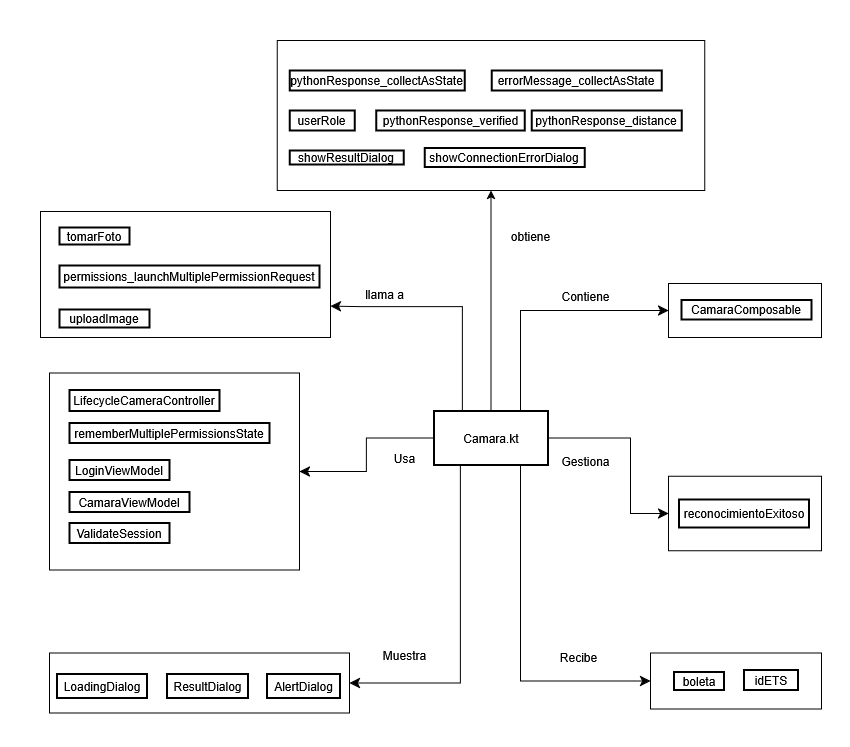
\includegraphics[width=0.9\textwidth]{DiagramasMoviles/DCM (14)}
		\caption{Diagrama de componentes para CamaraScreen.kt .}
		\label{fig:Componentes_2}
	\end{center}
\end{figure}

\newpage

\subsection{Diagrama de Componentes de ChatScreen.kt}

La Figura \ref{fig:Componentes_3} muestra el diagrama de componentes para ChatScreen.kt que es un composable que contiene una pantalla que muestra el chat de mensajes que pueden usar los usuarios.

\begin{figure}[htbp!]
	\begin{center}
		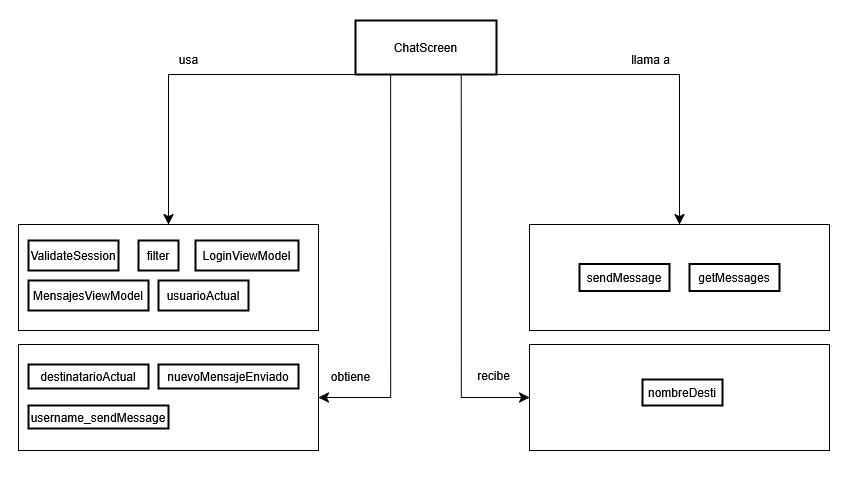
\includegraphics[width=0.9\textwidth]{DiagramasMoviles/DCM (15)}
		\caption{Diagrama de componentes para ChatScreen.kt .}
		\label{fig:Componentes_3}
	\end{center}
\end{figure}

\newpage

\subsection{Diagrama de Componentes de ConsultarScreen.kt}

La Figura \ref{fig:Componentes_4} muestra el diagrama de componentes para ConsultarScreen.kt que es un composable que contiene a la \IUref{IU12}{Pantalla Buscar alumno}, que muestra la lista de los alumnos inscritos a un ETS para el personal de seguridad y le permite filtrarlos por nombre o boleta.

\begin{figure}[htbp!]
	\begin{center}
		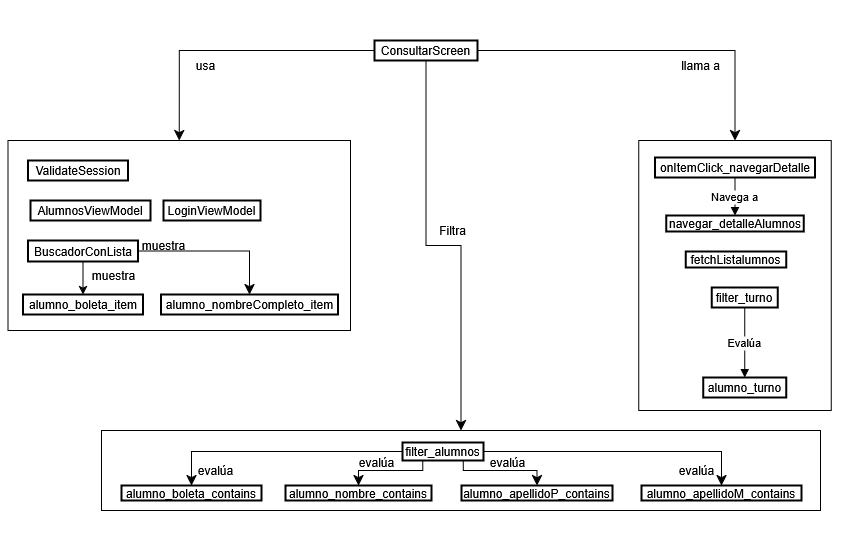
\includegraphics[width=0.9\textwidth]{DiagramasMoviles/DCM (16)}
		\caption{Diagrama de componentes para ConsultarScreen.kt .}
		\label{fig:Componentes_4}
	\end{center}
\end{figure}

\newpage

\subsection{Diagrama de Componentes de CredencialDaeScreen.kt}

La Figura \ref{fig:Componentes_5} muestra el diagrama de componentes para CredencialDaeScreen.kt que es un composable que contiene a la \IUref{IU11}{Pantalla Credencial del alumno}, que muestra la comparación de la credencial de la DAE con la credencial creada por el sistema.

\begin{figure}[htbp!]
	\begin{center}
		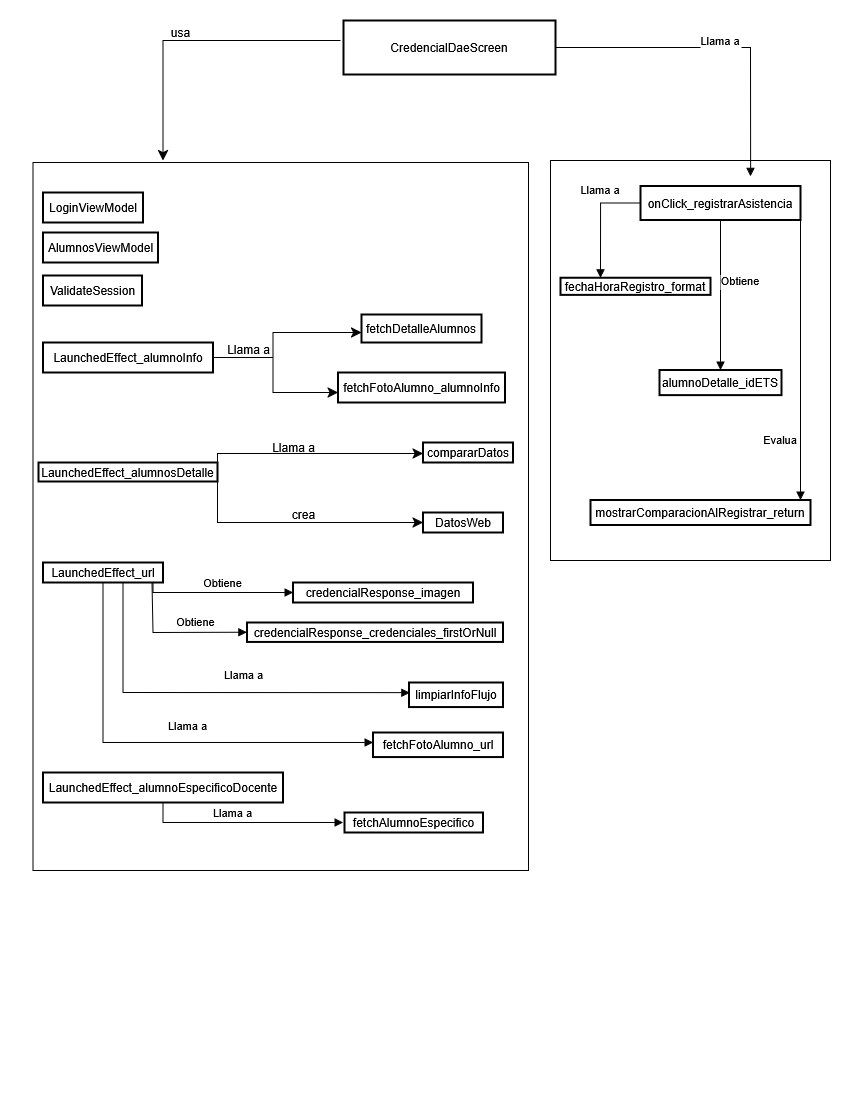
\includegraphics[width=0.9\textwidth]{DiagramasMoviles/DCM (17)}
		\caption{Diagrama de componentes para CredencialDaeScreen.kt .}
		\label{fig:Componentes_5}
	\end{center}
\end{figure}

\newpage

\subsection{Diagrama de Componentes de DetallesAlumnosScreen.kt}

La Figura \ref{fig:Componentes_6} muestra el diagrama de componentes para DetallesAlumnosScreen.kt que es un composable que contiene a la \IUref{IU11}{Pantalla Credencial del alumno}, que en este caso muestra la información relevante del alumno.

\begin{figure}[htbp!]
	\begin{center}
		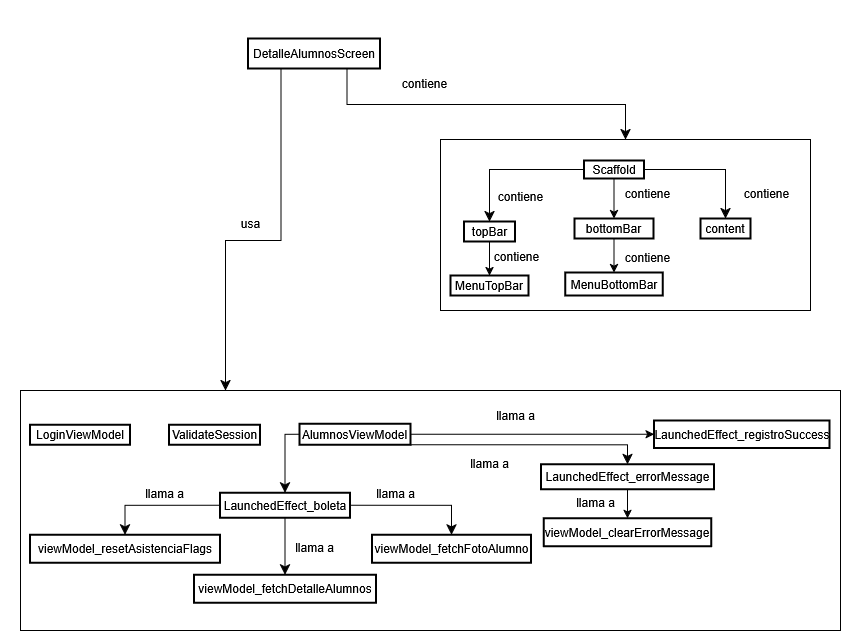
\includegraphics[width=0.9\textwidth]{DiagramasMoviles/DCM (19)}
		\caption{Diagrama de componentes para DetallesAlumnosScreen.kt .}
		\label{fig:Componentes_6}
	\end{center}
\end{figure}

\newpage

\subsection{Diagrama de Componentes de EtsDetailScreen.kt}

La Figura \ref{fig:Componentes_7} muestra el diagrama de componentes para EtsDetailScreen.kt que es un composable que contiene a la \IUref{IU06}{Pantalla Información de ETS} y \IUref{IU16}{Pantalla Información de ETS del alumno}, que muestra la información del ETS elegido por el usuario.

\begin{figure}[htbp!]
	\begin{center}
		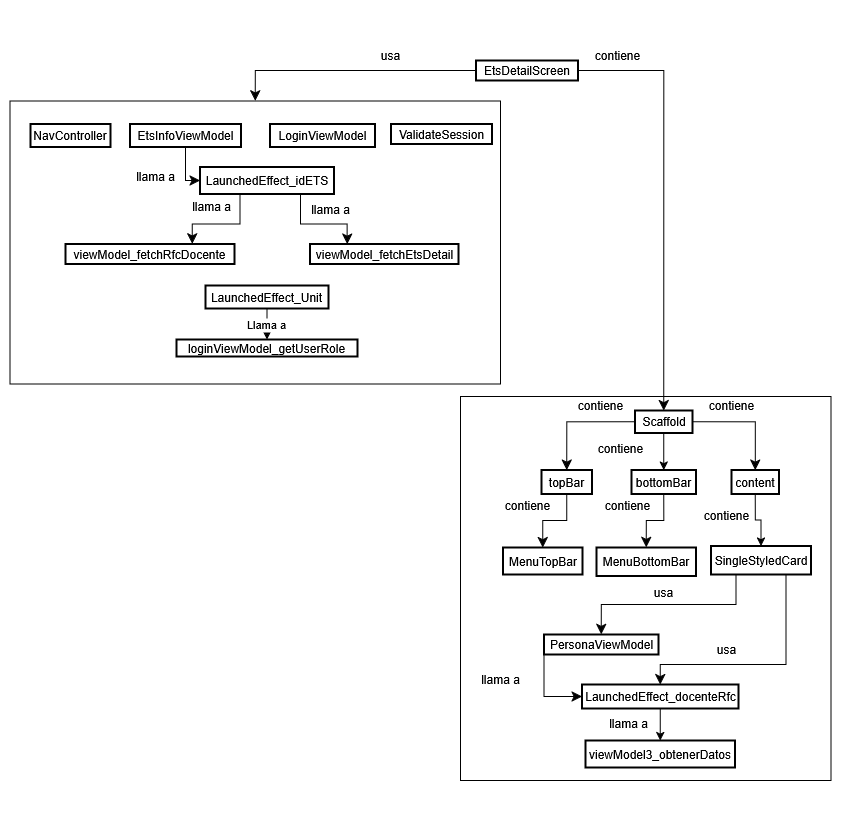
\includegraphics[width=0.9\textwidth]{DiagramasMoviles/DCM (20)}
		\caption{Diagrama de componentes para EtsDetailScreen.kt .}
		\label{fig:Componentes_7}
	\end{center}
\end{figure}

\newpage

\subsection{Diagrama de Componentes de EtsInscriptionProcessScreen.kt}

La Figura \ref{fig:Componentes_8} muestra el diagrama de componentes para ETSInscriptionProcessScreen.kt que es un composable que contiene a la \IUref{IU18}{Pantalla de Detalles del proceso de ETS}, que muestra la información necesaria para inscribirse a un ETS.

\begin{figure}[htbp!]
	\begin{center}
		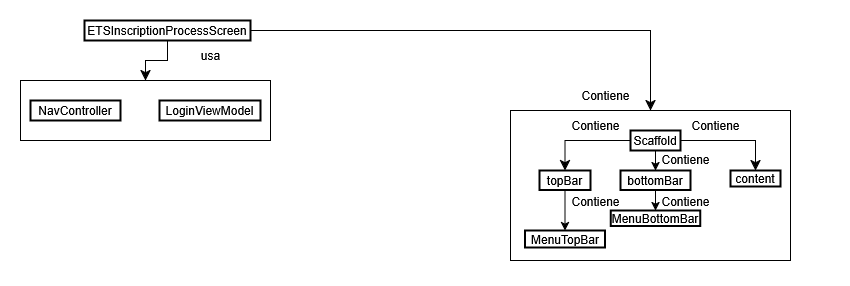
\includegraphics[width=0.9\textwidth]{DiagramasMoviles/DCM (21)}
		\caption{Diagrama de componentes para ETSInscriptionProcessScreen.kt .}
		\label{fig:Componentes_8}
	\end{center}
\end{figure}

\newpage

\subsection{Diagrama de Componentes de EtsListScreen.kt}

La Figura \ref{fig:Componentes_9} muestra el diagrama de componentes para EtsListScreen.kt que es un composable que contiene a la \IUref{IU05}{Pantalla Consultar ETS}, que muestra la lista de ETS del docente.

\begin{figure}[htbp!]
	\begin{center}
		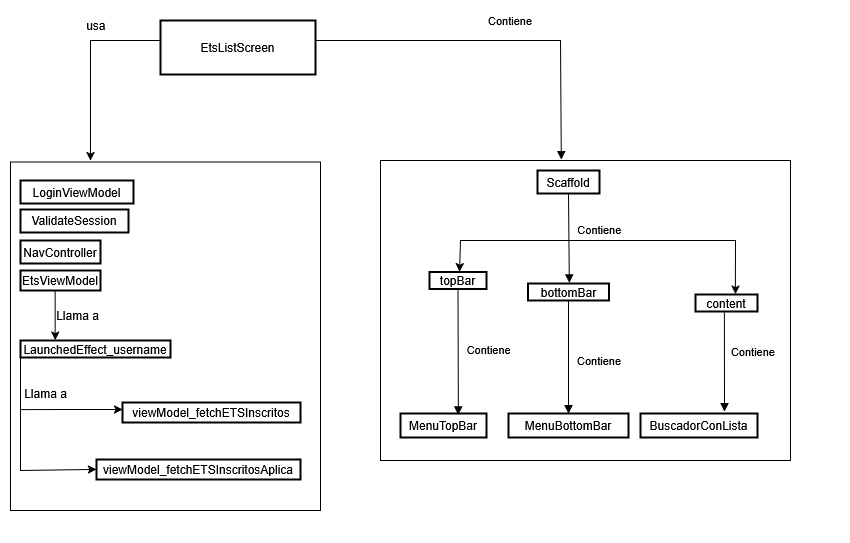
\includegraphics[width=0.9\textwidth]{DiagramasMoviles/DCM (22)}
		\caption{Diagrama de componentes para EtsListScreen.kt .}
		\label{fig:Componentes_9}
	\end{center}
\end{figure}

\newpage

\subsection{Diagrama de Componentes de EtsListScreenAlumno.kt}

La Figura \ref{fig:Componentes_10} muestra el diagrama de componentes para EtsListScreenAlumno.kt que es un composable que contiene a la \IUref{IU05}{Pantalla Consultar ETS}, que muestra la lista de ETS del alumno.

\begin{figure}[htbp!]
	\begin{center}
		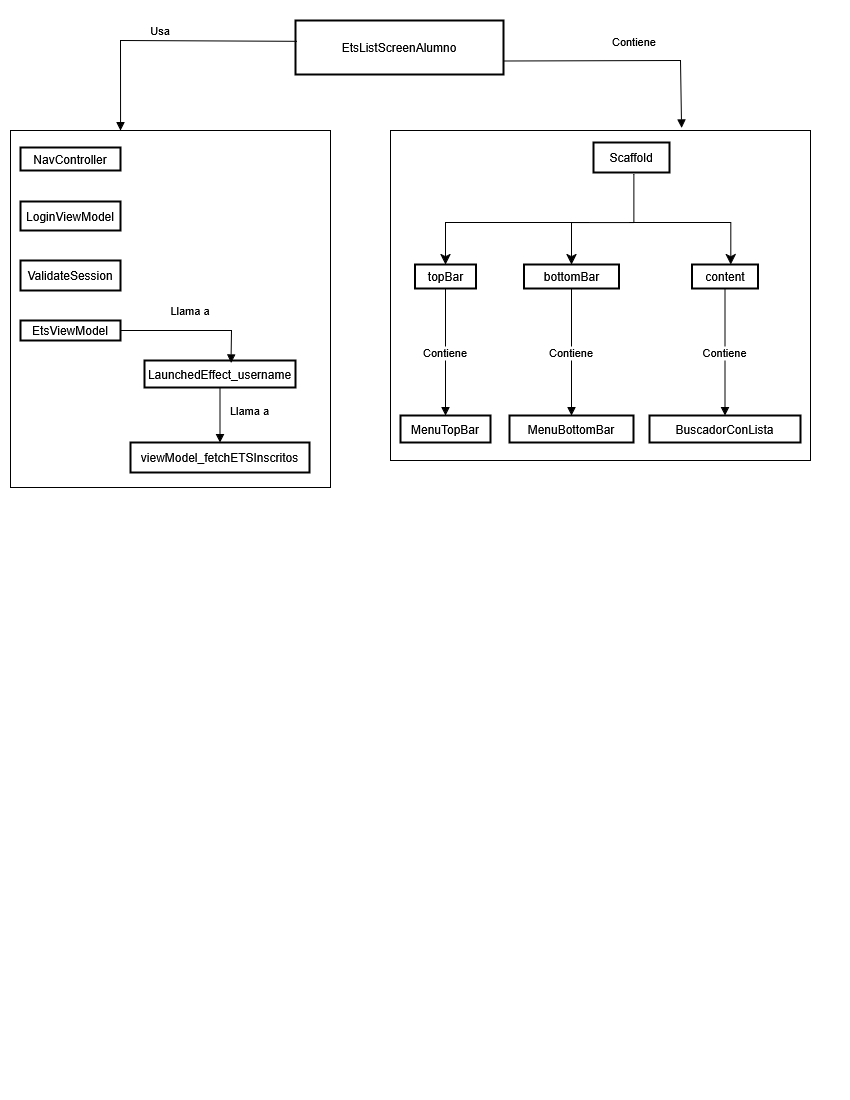
\includegraphics[width=0.9\textwidth]{DiagramasMoviles/DCM (23)}
		\caption{Diagrama de componentes para EtsListScreenAlumno.kt .}
		\label{fig:Componentes_10}
	\end{center}
\end{figure}

\newpage

\subsection{Diagrama de Componentes de InformacionAlumno.kt}

La Figura \ref{fig:Componentes_11} muestra el diagrama de componentes para InformacionAlumno.kt que es un composable que contiene a la \IUref{IUE07}{Creación del reporte}, que se utiliza para la creación de reportes y a su vez muestra la información esencial del alumno seleccionado.

\begin{figure}[htbp!]
	\begin{center}
		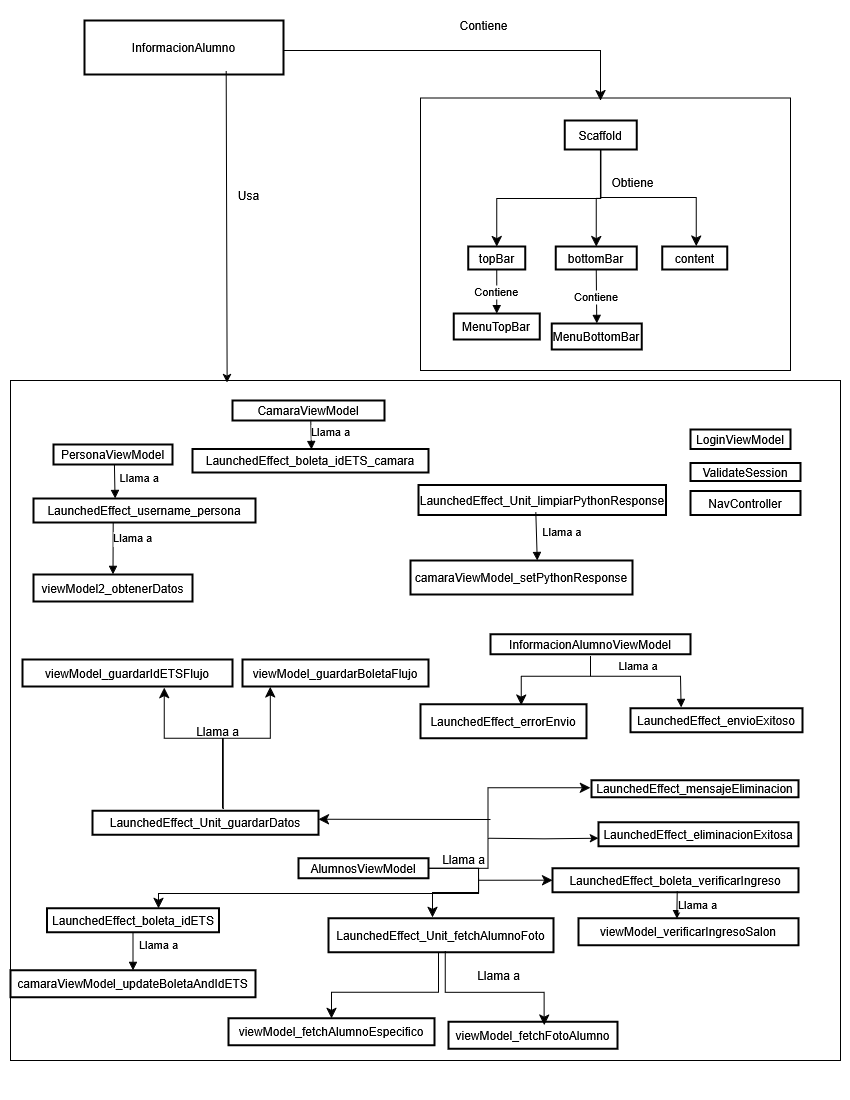
\includegraphics[width=0.7\textwidth]{DiagramasMoviles/DCM (24)}
		\caption{Diagrama de componentes para InformacionAlumno.kt .}
		\label{fig:Componentes_11}
	\end{center}
\end{figure}

\newpage

\subsection{Diagrama de Componentes de ListaAlumnosScreen.kt}

La Figura \ref{fig:Componentes_12} muestra el diagrama de componentes para ListaAlumnosScreen.kt que es un composable que contiene a la \IUref{IU08}{Pantalla Lista de asistencia de ETS}, que es la que le muestra la lista de alumnos inscritos a un ETS al docente, junto con su estado de asistencia con un icono.

\begin{figure}[htbp!]
	\begin{center}
		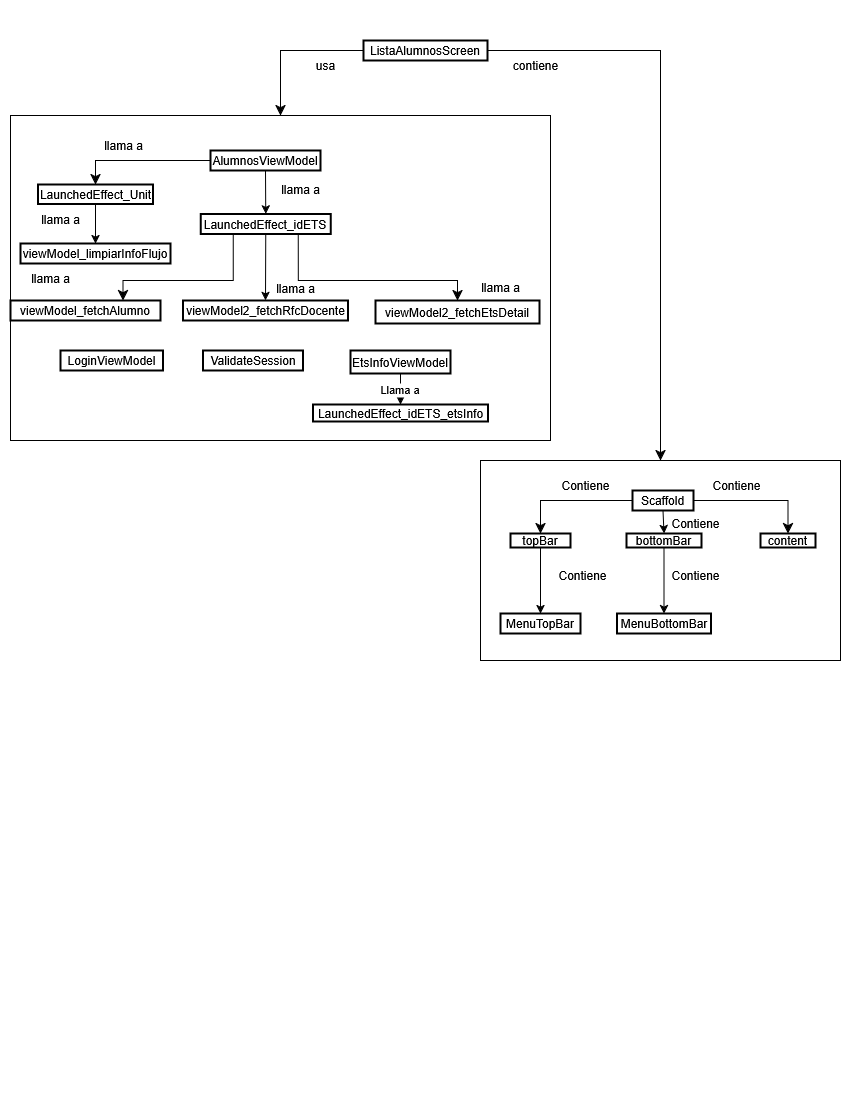
\includegraphics[width=0.9\textwidth]{DiagramasMoviles/DCM (25)}
		\caption{Diagrama de componentes para ListaAlumnosScreen.kt .}
		\label{fig:Componentes_12}
	\end{center}
\end{figure}

\newpage

\subsection{Diagrama de Componentes de ListadoSolicitudesReemplazo.kt}

La Figura \ref{fig:Componentes_13} muestra el diagrama de componentes para ListadoSolicitudesReemplazo.kt que es un composable que contiene una pantalla dedica a la visualización de las solicitudes de reemplazo y sus estados de aceptación o denegación. 

\begin{figure}[htbp!]
	\begin{center}
		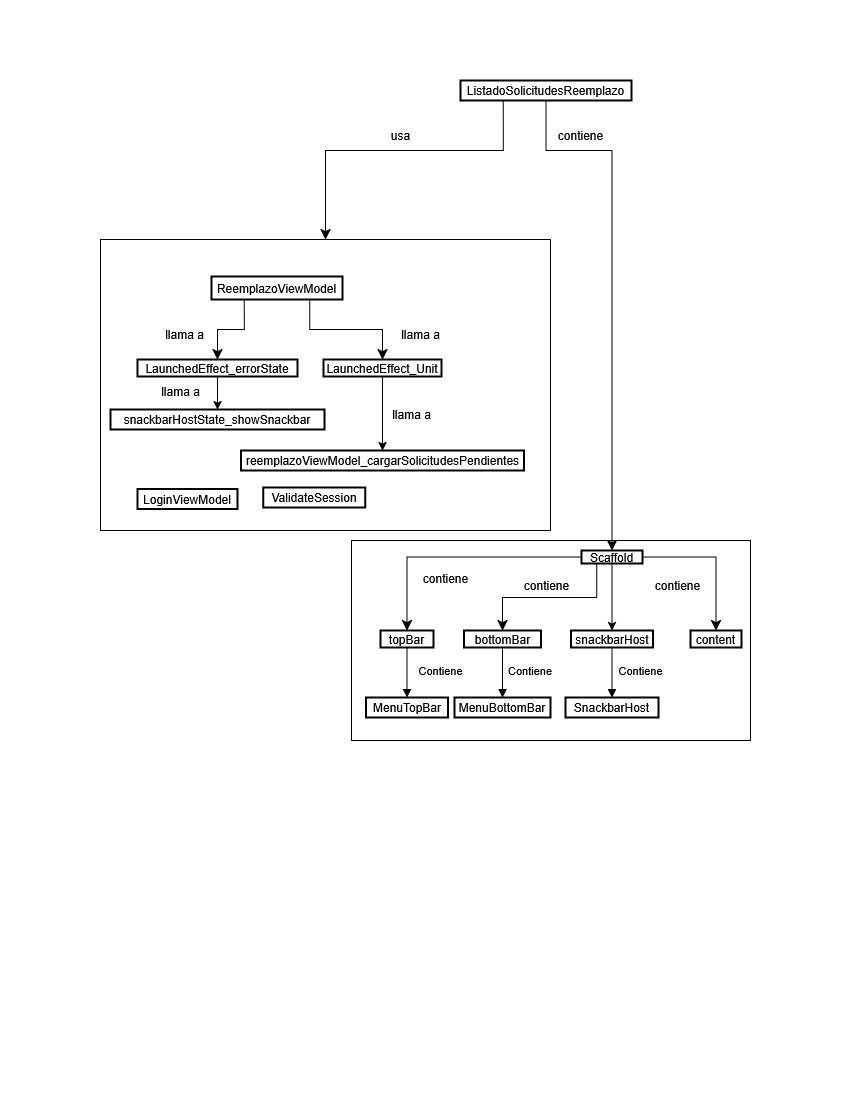
\includegraphics[width=0.9\textwidth]{DiagramasMoviles/DCM (26)}
		\caption{Diagrama de componentes para ListadoSolicitudesReemplazo.kt .}
		\label{fig:Componentes_13}
	\end{center}
\end{figure}

\newpage

\subsection{Diagrama de Componentes de LoginScreen.kt}

La Figura \ref{fig:Componentes_14} muestra el diagrama de componentes para LoginScreen.kt que es un composable que contiene a la \IUref{IU01}{Pantalla Iniciar sesión del sistema móvil}, que es el login de la aplicación móvil.

\begin{figure}[htbp!]
	\begin{center}
		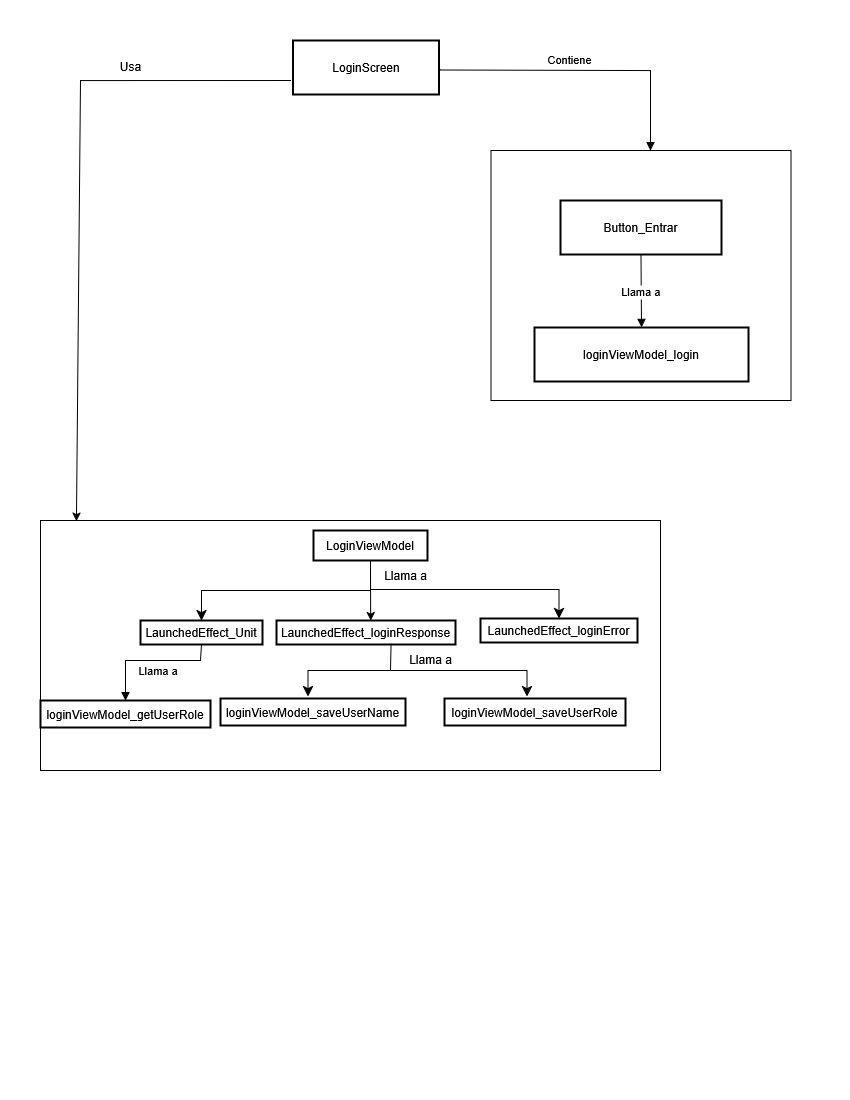
\includegraphics[width=0.9\textwidth]{DiagramasMoviles/DCM (27)}
		\caption{Diagrama de componentes para LoginScreen.kt .}
		\label{fig:Componentes_14}
	\end{center}
\end{figure}

\newpage

\subsection{Diagrama de Componentes de MensajesScreen.kt}

La Figura \ref{fig:Componentes_15} muestra el diagrama de componentes para MensajesScreen.kt que es un composable que es la pantalla donde se ven los mensaje específicos mandados a otro usuario.

\begin{figure}[htbp!]
	\begin{center}
		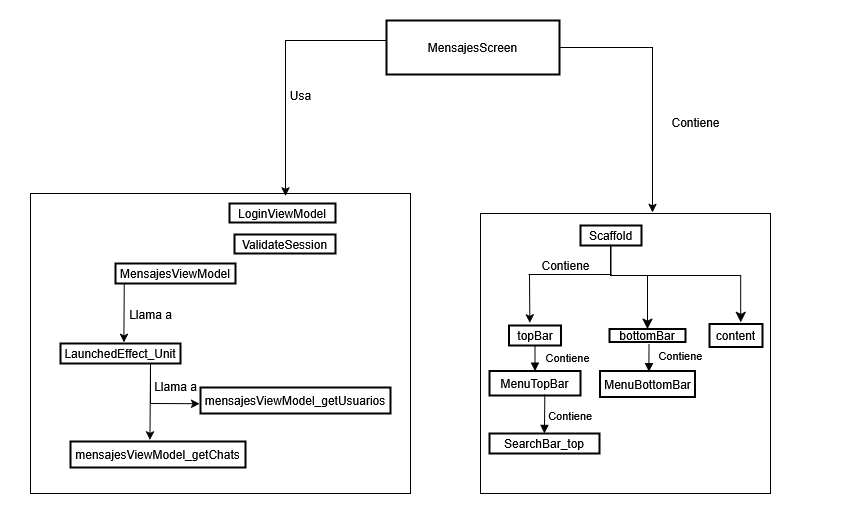
\includegraphics[width=0.9\textwidth]{DiagramasMoviles/DCM (28)}
		\caption{Diagrama de componentes para MensajesScreen.kt .}
		\label{fig:Componentes_15}
	\end{center}
\end{figure}

\newpage

\subsection{Diagrama de Componentes de QRScannerScreen.kt}

La Figura \ref{fig:Componentes_16} muestra el diagrama de componentes para QRScannerScreen.kt que es un composable que contiene a la \IUref{IU10}{Pantalla Código QR}, que muestra la cámara para poder escanear el código QR de la credencial del alumno.

\begin{figure}[htbp!]
	\begin{center}
		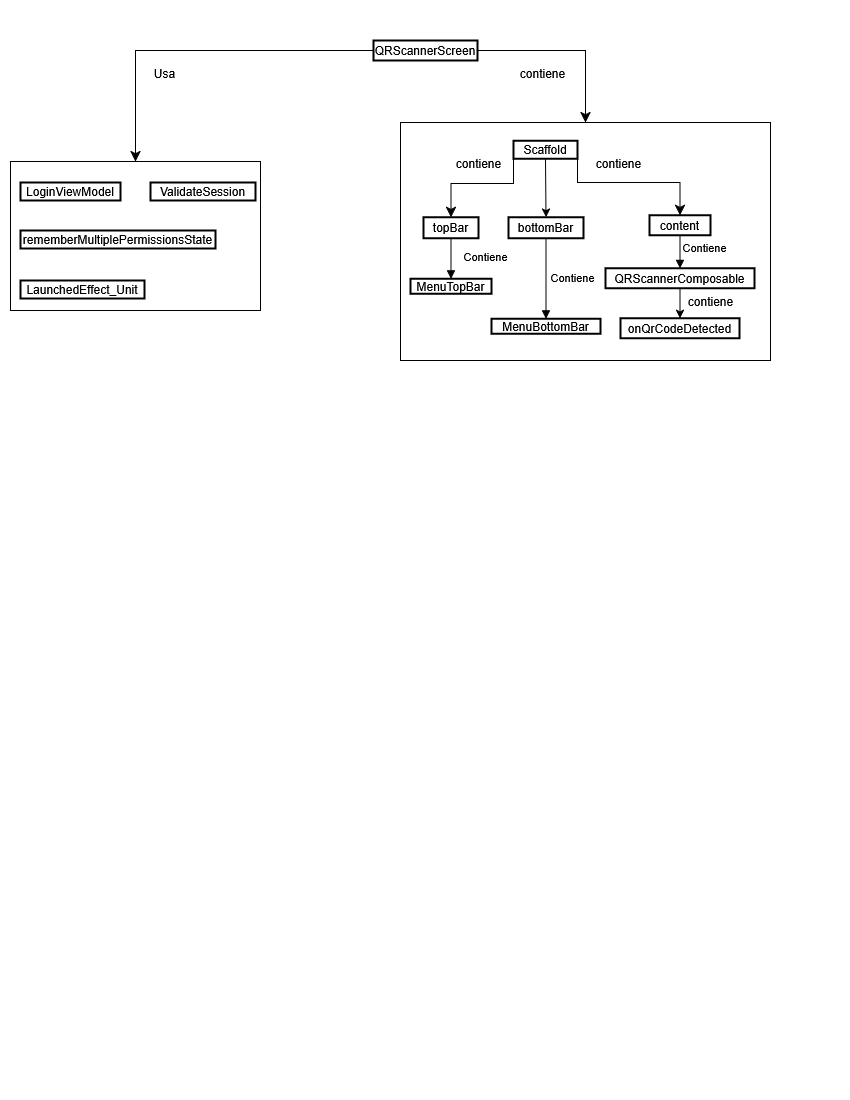
\includegraphics[width=0.9\textwidth]{DiagramasMoviles/DCM (29)}
		\caption{Diagrama de componentes para QRScannerScreen.kt .}
		\label{fig:Componentes_16}
	\end{center}
\end{figure}

\newpage

\subsection{Diagrama de Componentes de ReporteScreen.kt}

La Figura \ref{fig:Componentes_17} muestra el diagrama de componentes para ReporteScreen.kt que es un composable que contiene a la \IUref{IU20}{Pantalla Reporte del Alumno}, que es donde el docente puede revisar el reporte de la asistencia del alumno.

\begin{figure}[htbp!]
	\begin{center}
		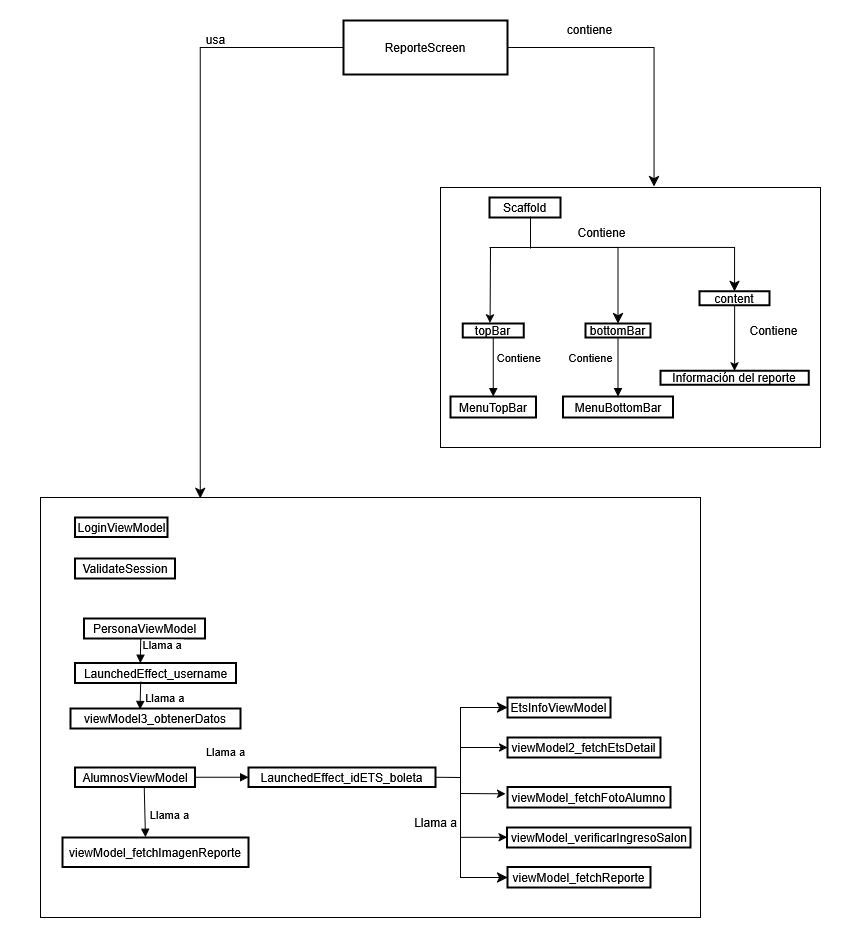
\includegraphics[width=0.7\textwidth]{DiagramasMoviles/DCM (30)}
		\caption{Diagrama de componentes para ReporteScreen.kt .}
		\label{fig:Componentes_17}
	\end{center}
\end{figure}

\newpage

\subsection{Diagrama de Componentes de ScreenAsignarremplazo.kt}

La Figura \ref{fig:Componentes_18} muestra el diagrama de componentes para ScreenAsignarremplazo.kt que es un composable que contiene a la pantalla \IUref{IU09}{Asignar docente de remplazo}, que es donde el jefe de departamento y/o el presidente de academia pueden responder a las solicitudes de reemplazo.

\begin{figure}[htbp!]
	\begin{center}
		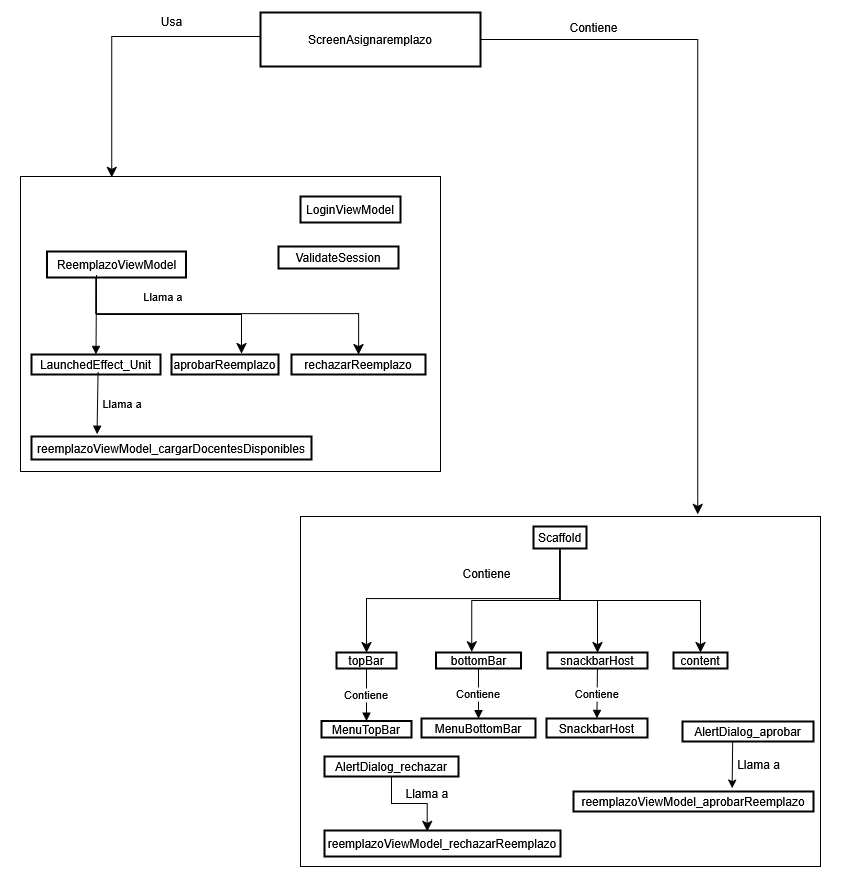
\includegraphics[width=0.9\textwidth]{DiagramasMoviles/DCM (31)}
		\caption{Diagrama de componentes para ScreenAsignarremplazo.kt .}
		\label{fig:Componentes_18}
	\end{center}
\end{figure}

\newpage

\subsection{Diagrama de Componentes de SolicitarReemplazo.kt}

La Figura \ref{fig:Componentes_19} muestra el diagrama de componentes para SolicitarReemplazo.kt que es un composable que contiene a la \IUref{IU07}{Pantalla de Solicitar remplazo}, que es donde el docente puede pedir un reemplazo como aplacador del ETS.

\begin{figure}[htbp!]
	\begin{center}
		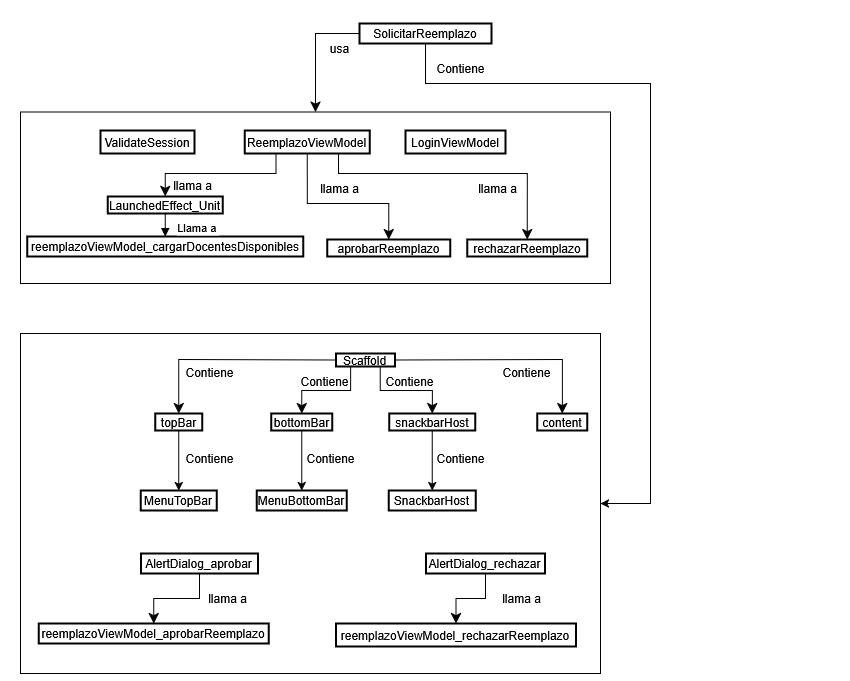
\includegraphics[width=0.9\textwidth]{DiagramasMoviles/DCM (32)}
		\caption{Diagrama de componentes para SolicitarReemplazo.kt .}
		\label{fig:Componentes_19}
	\end{center}
\end{figure}

\newpage

\subsection{Diagrama de Componentes de WelcomeScreen.kt}

La Figura \ref{fig:Componentes_20} muestra el diagrama de componentes para WelcomeScreen.kt que es un composable que contiene a la \IUref{IUE02}{Pantalla de saludo del personal de seguridad}, que es la pantalla de inicio del personal de seguridad (donde pude seleccionar la operación que quiere realizar y ver un saludo con su nombre).

\begin{figure}[htbp!]
	\begin{center}
		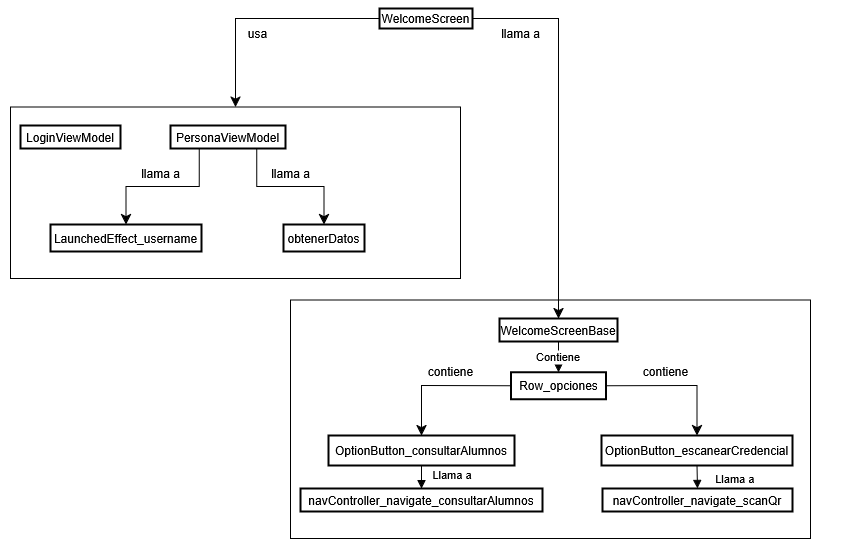
\includegraphics[width=0.9\textwidth]{DiagramasMoviles/DCM (33)}
		\caption{Diagrama de componentes para WelcomeScreen.kt .}
		\label{fig:Componentes_20}
	\end{center}
\end{figure}

\newpage

\subsection{Diagrama de Componentes de WelcomeScreenAcademico.kt}

La Figura \ref{fig:Componentes_21} muestra el diagrama de componentes para WelcomeScreenAcademico.kt que es un composable que contiene a la pantalla \IUref{IUE06}{saludo del presidente de academia y el jefe de departamento}, que es la pantalla de inicio del jefe de departamento y/o el presidente de academia (donde pude seleccionar la operación que quiere realizar y ver un saludo con su nombre).

\begin{figure}[htbp!]
	\begin{center}
		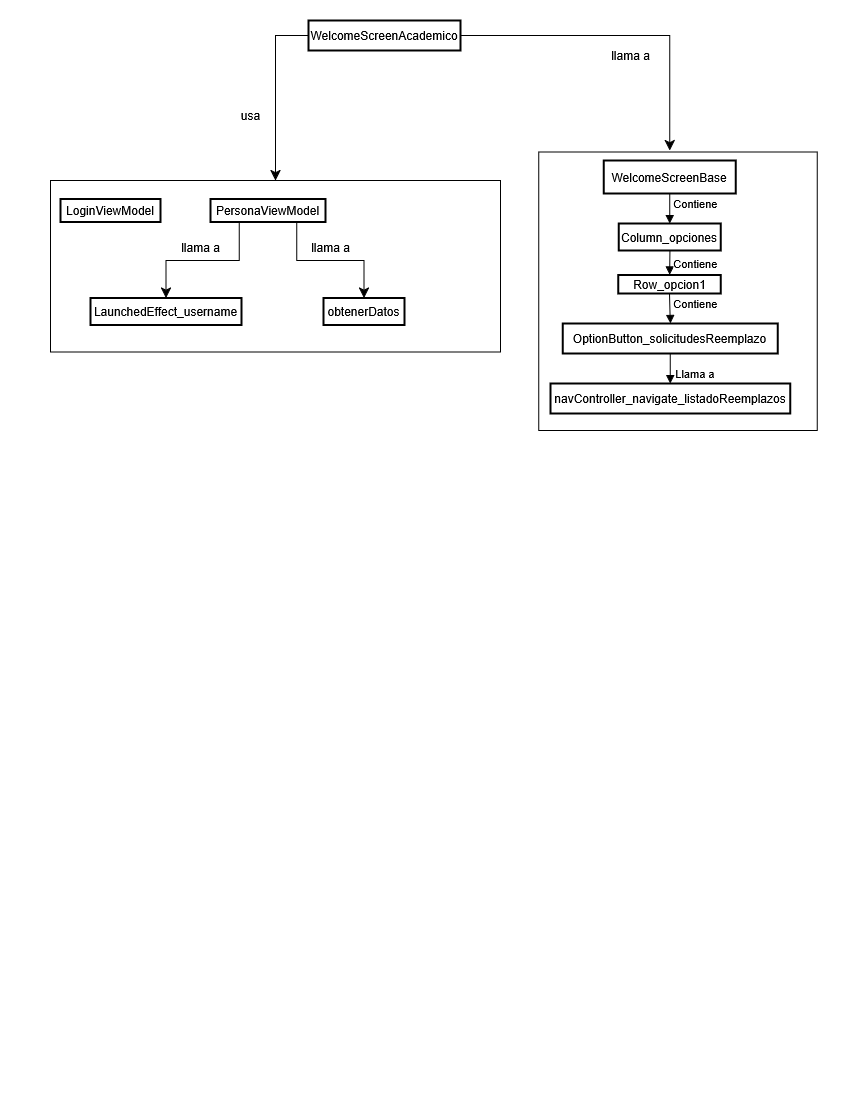
\includegraphics[width=0.9\textwidth]{DiagramasMoviles/DCM (34)}
		\caption{Diagrama de componentes para WelcomeScreenAcademico.kt .}
		\label{fig:Componentes_21}
	\end{center}
\end{figure}

\newpage

\subsection{Diagrama de Componentes de WelcomeScreenAlumno.kt}

La Figura \ref{fig:Componentes_22} muestra el diagrama de componentes para WelcomeScreenAlumno.kt que es un composable que contiene a la pantalla \IUref{IUE03}{Pantalla saludo del alumno}, que es la pantalla de inicio del Alumno (donde pude seleccionar la operación que quiere realizar y ver un saludo con su nombre).

\begin{figure}[htbp!]
	\begin{center}
		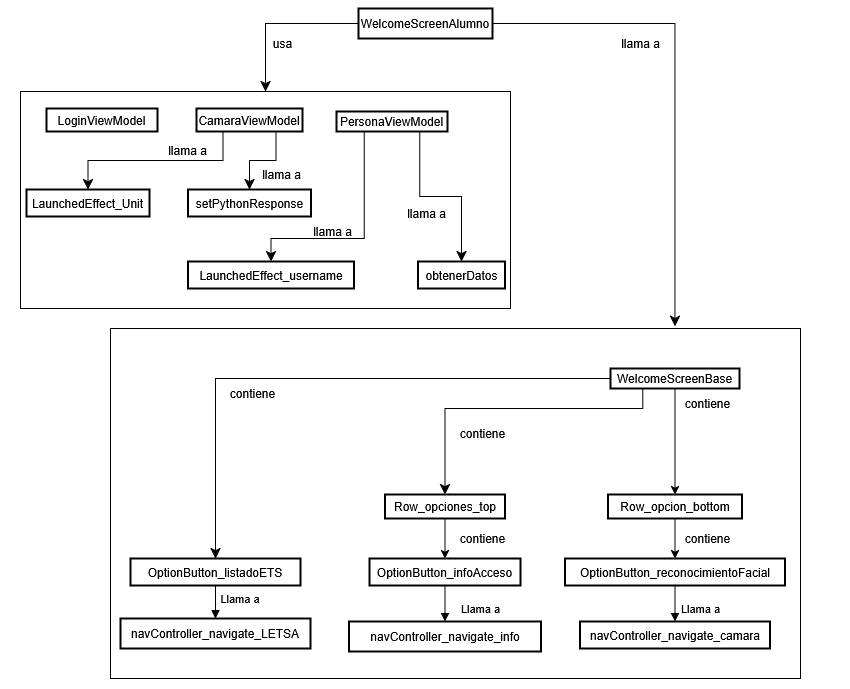
\includegraphics[width=0.9\textwidth]{DiagramasMoviles/DCM (35)}
		\caption{Diagrama de componentes para WelcomeScreenAlumno.kt .}
		\label{fig:Componentes_22}
	\end{center}
\end{figure}

\newpage

\subsection{Diagrama de Componentes de WelcomeScreenDocente.kt}

La Figura \ref{fig:Componentes_23} muestra el diagrama de componentes para WelcomeScreenDocente.kt que es un composable que contiene a la pantalla \IUref{IUE01}{Pantalla saludo de docente}, que es la pantalla de inicio del Docente (donde pude seleccionar la operación que quiere realizar y ver un saludo con su nombre).

\begin{figure}[htbp!]
	\begin{center}
		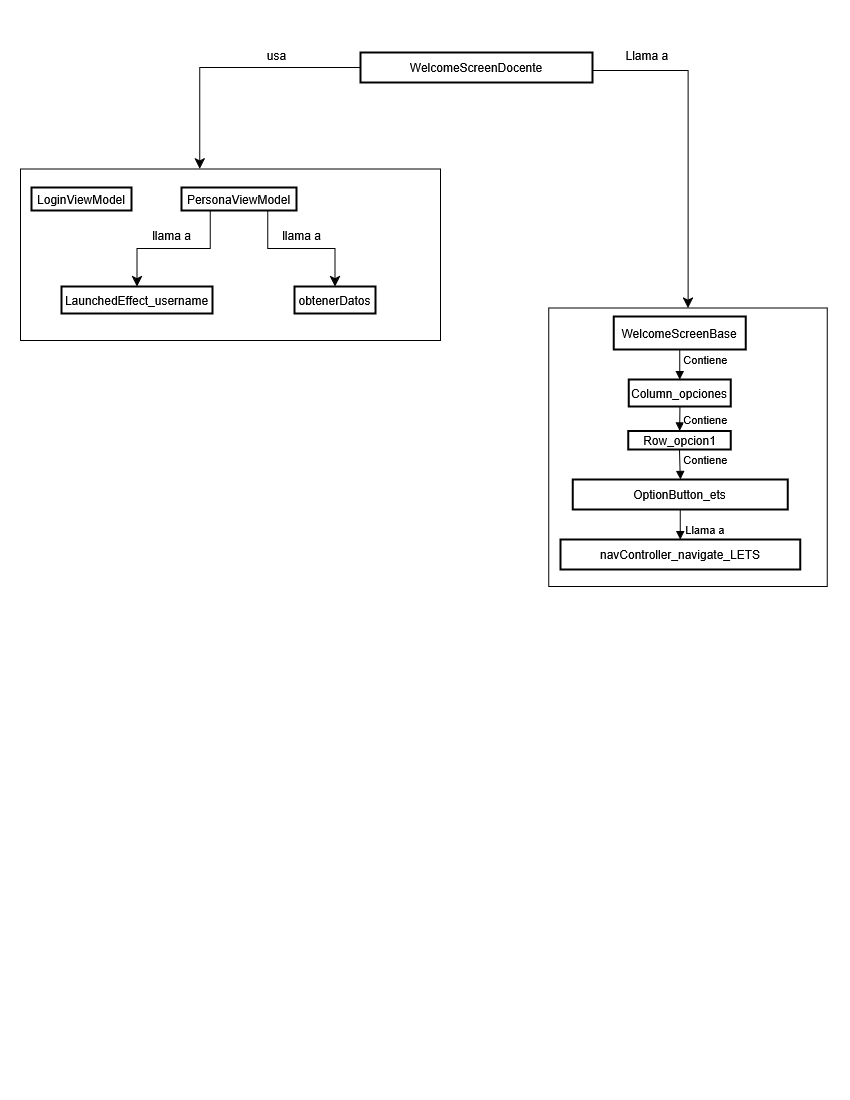
\includegraphics[width=0.9\textwidth]{DiagramasMoviles/DCM (36)}
		\caption{Diagrama de componentes para WelcomeScreenDocente.kt .}
		\label{fig:Componentes_23}
	\end{center}
\end{figure}

\newpage


%\section{Diagrama de clases}

%En la figura \ref{fig:Diagrama de clases} se muestra el diagrama de clases del sistema, en el cual se establecen las clases que tenemos contempladas para ser implementadas en la creación del sistema, a su vez en este se muestran las relaciones entre las clases, los atributos que estes clases contienen y los procesos que llevaran a cabo.


%\begin{figure}[htbp!]
%	\begin{center}
%		\includegraphics[width=1\textwidth]{Clases/Clases2}
%		\caption{Diagrama de clases.}
%		\label{fig:Diagrama de clases}
%	\end{center}
%\end{figure}


\section{Diagramas de secuencia}

A continuación, se presentan los diagramas de secuencia identificados para para la propuesta de solución presentada en este documento.
En ellos se busca ilustrar el funcionamiento dinamico del sistema y modelar las interacciones entre los distintos componentes y actores dependiendo de los casos de uso descritos en el capitulo 4. 
Cada diagrama representa el flujo de mensajes e información entre los actores y las capas de la aplicación en función de la arquitectura de una aplicación basada en Spring boot.

\subsection{SE-01 Iniciar sesión del sistema móvil}

\begin{figure}[htbp!]
	\begin{center}
		\fbox{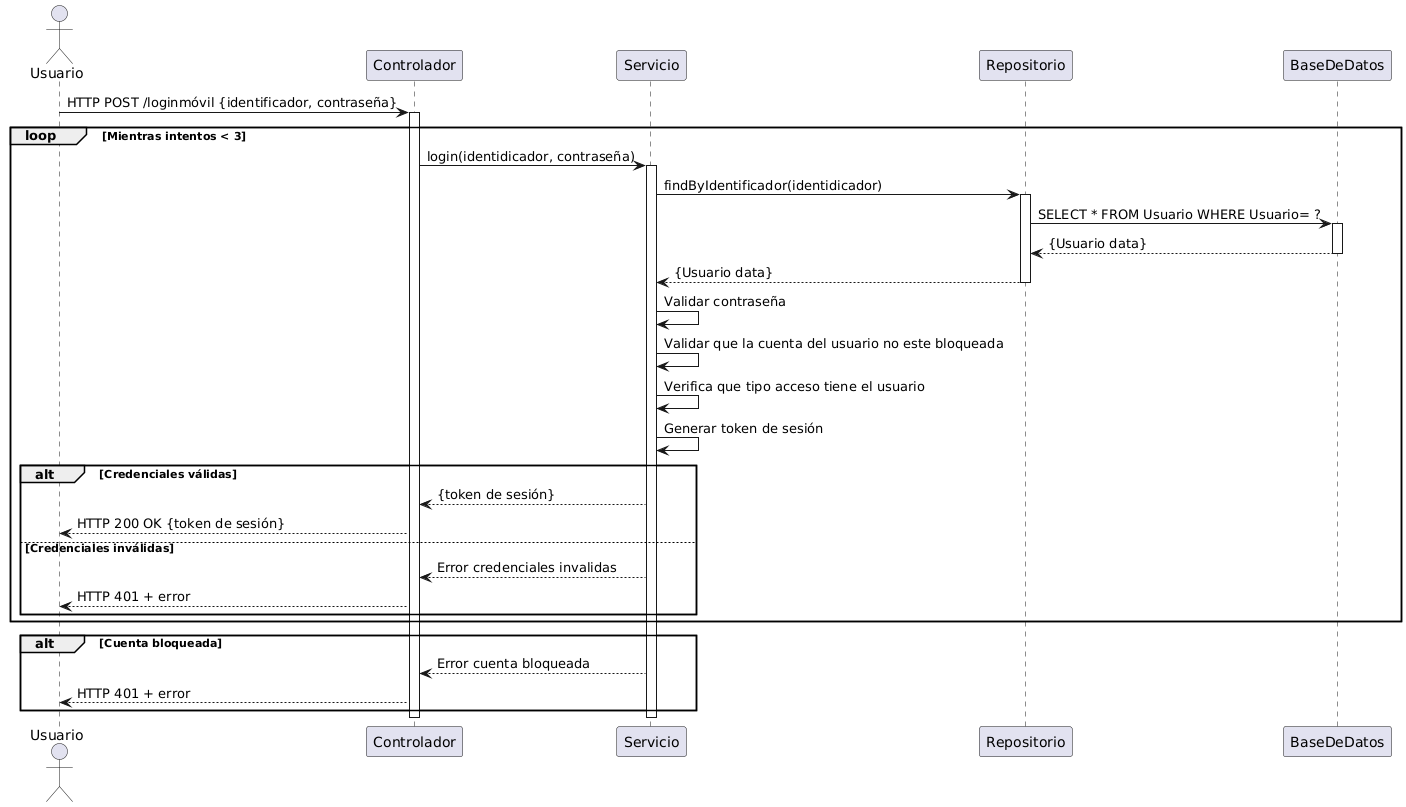
\includegraphics[width=1\textwidth]{Secuencia/CU-01.png}}
		\caption{Diagrama de secuencia del caso de uso número 01 (Iniciar sesión del sistema móvil).}
		\label{fig:Diagrama de secuencia CU-01}
	\end{center}
\end{figure}

En el diagrama de secuencia \ref{fig:Diagrama de secuencia CU-01} de secuencia se describe el proceso planeado para el caso de uso \hyperlink{CU-01}{CU-01 Iniciar sesión del sistema móvil}, mostrando las interacciones que tendrá con la vista, el controlador, el servicio, el repositorio y la base de datos.

\newpage

\subsection{SE-02 Consultar calendario escolar}

\begin{figure}[htbp!]
	\begin{center}
		\fbox{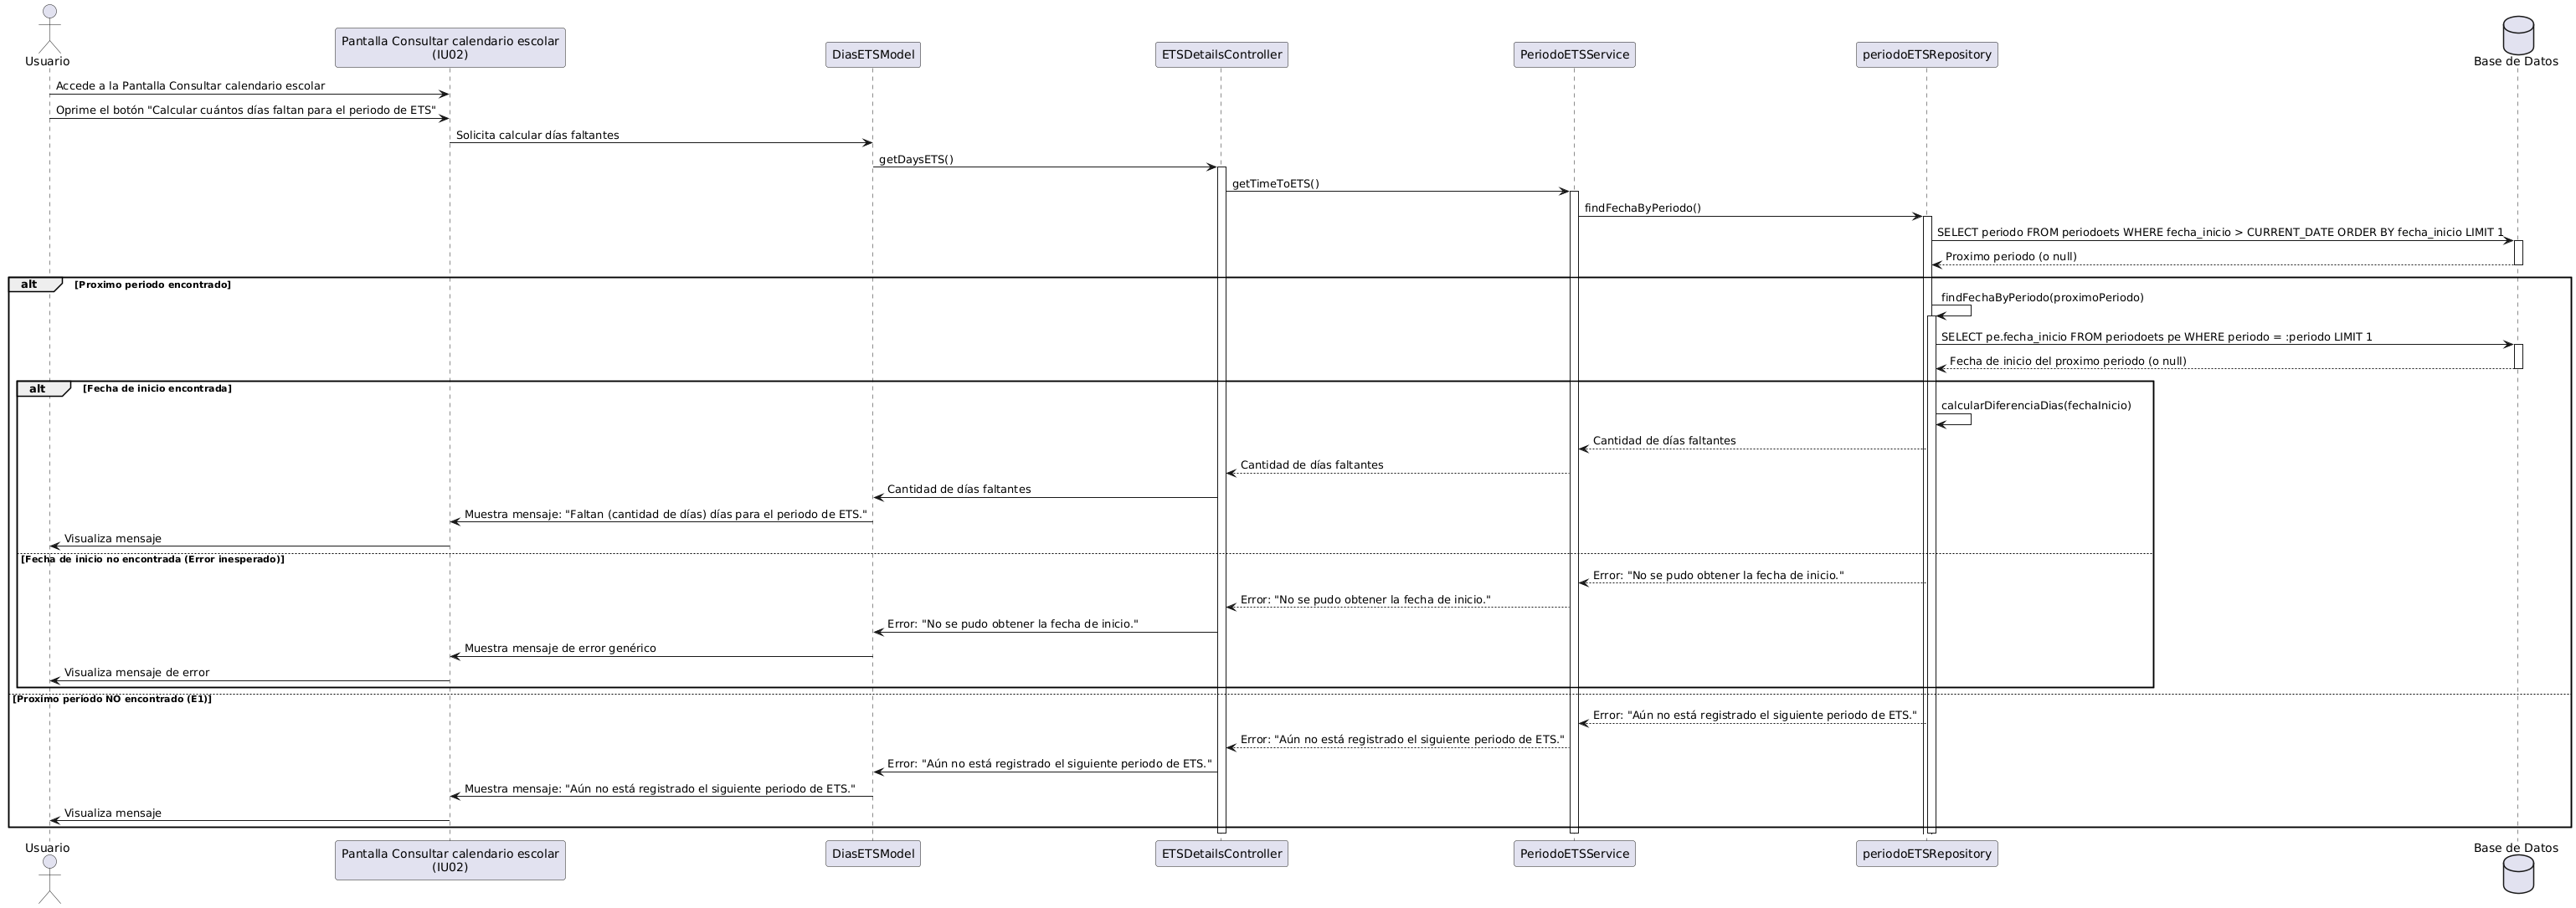
\includegraphics[width=1\textwidth]{Secuencia/CU-02.png}}
		\caption{Diagrama de secuencia del caso de uso número 02 (Consultar calendario escolar).}
		\label{fig:Diagrama de secuencia CU-02}
	\end{center}
\end{figure}

En el diagrama de secuencia \ref{fig:Diagrama de secuencia CU-02} se describe el proceso planeado para el caso de uso \hyperlink{CU-02}{CU-02 Consultar calendario escolar}, mostrando las interacciones que tendrá con la vista, el controlador, el servicio, el repositorio y la base de datos.

\newpage

\subsection{SE-03 Consultar notificaciones}

\begin{figure}[htbp!]
	\begin{center}
		\fbox{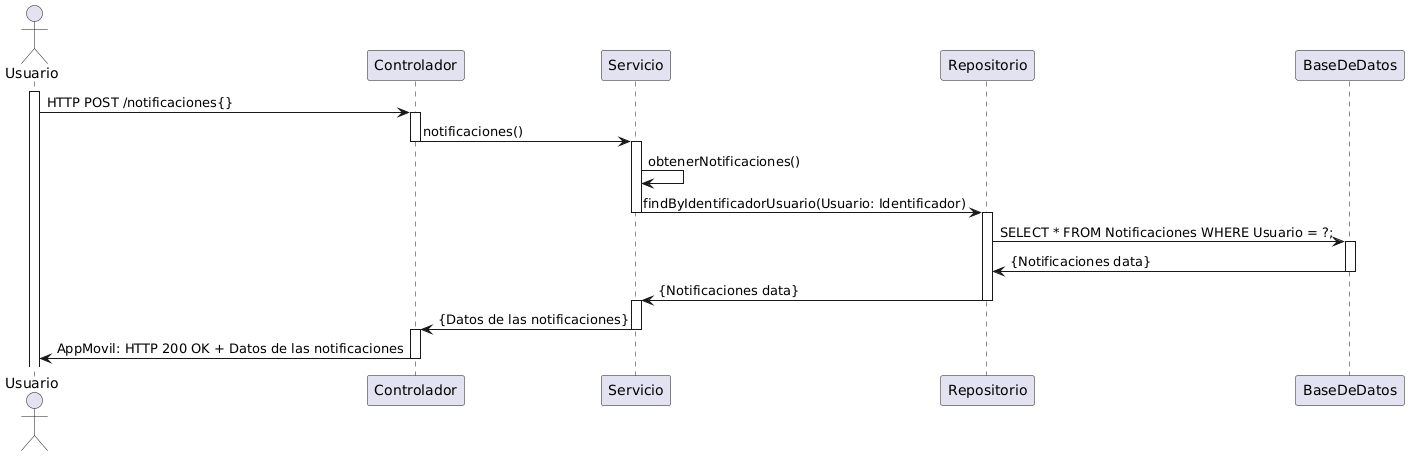
\includegraphics[width=1\textwidth]{Secuencia/CU-03.png}}
		\caption{Diagrama de secuencia del caso de uso número 03 (Consultar notificaciones).}
		\label{fig:Diagrama se secuencia CU-03}
	\end{center}
\end{figure}

En el diagrama de secuencia \ref{fig:Diagrama de secuencia CU-03} se describe el proceso planeado para el caso de uso \hyperlink{CU-03}{CU-03 Consultar notificaciones}, mostrando las interacciones que tendrá con la vista, el controlador, el servicio, el repositorio y la base de datos.

\newpage

\subsection{SE-04 Consultar periodos de ETS asignados al docente}

\begin{figure}[htbp!]
	\begin{center}
		\fbox{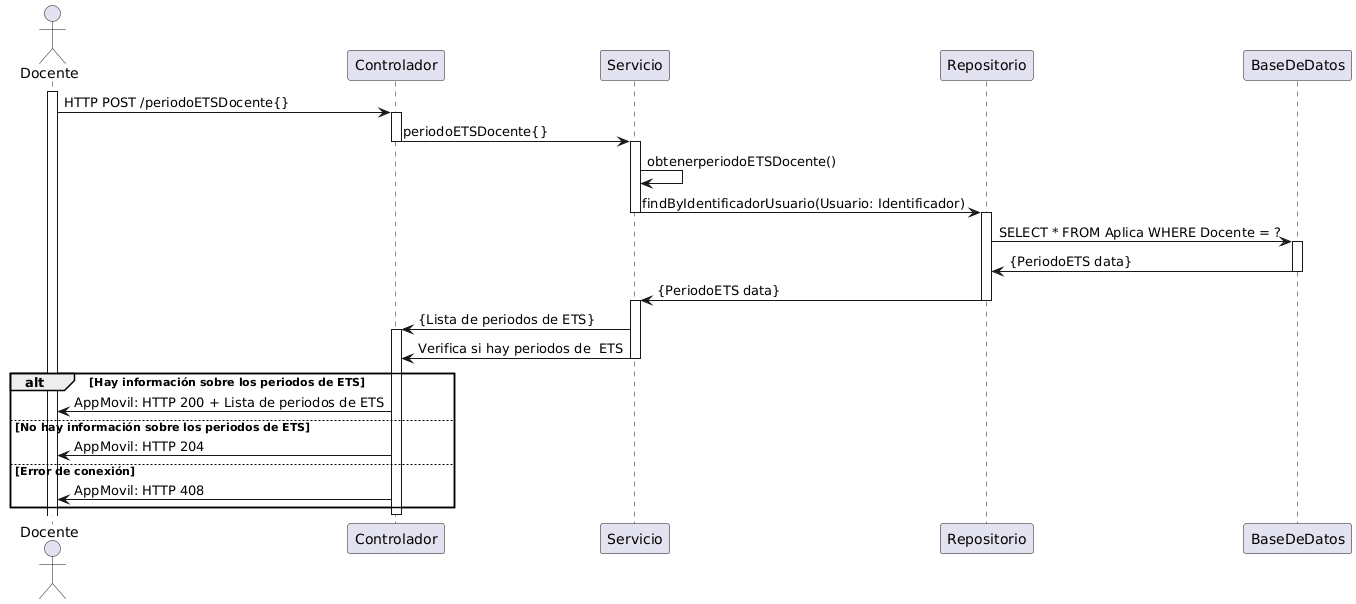
\includegraphics[width=1\textwidth]{Secuencia/CU-04.png}}
		\caption{Diagrama de secuencia del caso de uso número 04 (Consultar periodos de ETS asignados al docente).}
		\label{fig:Diagrama de secuencia CU-04}
	\end{center}
\end{figure}

En el diagrama de secuencia \ref{fig:Diagrama de secuencia CU-04} se describe el proceso planeado para el caso de uso \hyperlink{CU-04}{CU-04 Consultar periodos de ETS asignados al docente}, mostrando las interacciones que tendrá con la vista, el controlador, el servicio, el repositorio y la base de datos.

\newpage

\subsection{SE-05 Consultar ETS asignados}

\begin{figure}[htbp!]
	\begin{center}
		\fbox{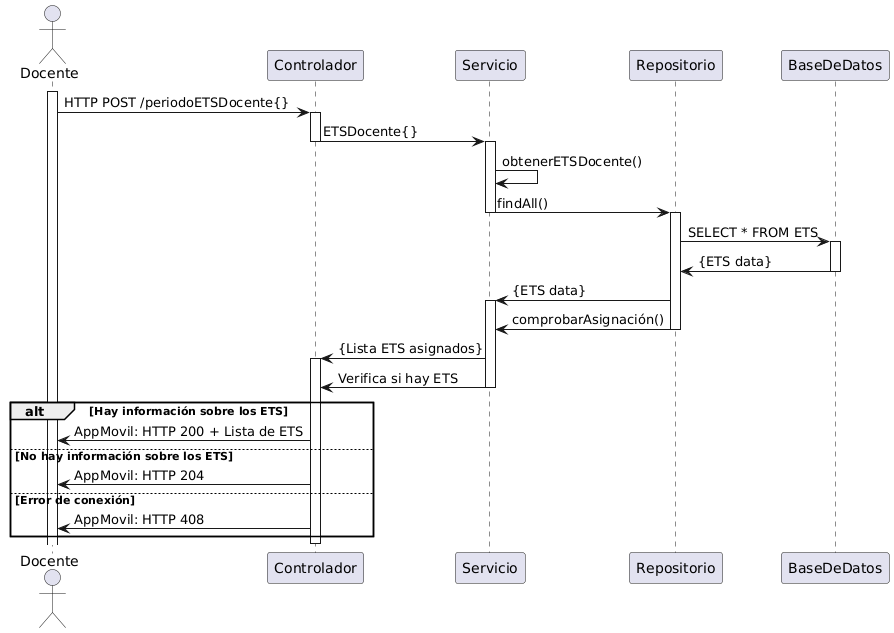
\includegraphics[width=1\textwidth]{Secuencia/CU-05.png}}
		\caption{Diagrama de secuencia del caso de uso número 05 (Consultar ETS asignados).}
		\label{fig:Diagrama de secuencia CU-05}
	\end{center}
\end{figure}

En el diagrama de secuencia \ref{fig:Diagrama de secuencia CU-05} se describe el proceso planeado para el caso de uso \hyperlink{CU-05}{CU-05 Consultar ETS asignados}, mostrando las interacciones que tendrá con la vista, el controlador, el servicio, el repositorio y la base de datos.

\newpage

\subsection{SE-06 Mostrar información de los ETS asignados}

\begin{figure}[htbp!]
	\begin{center}
		\fbox{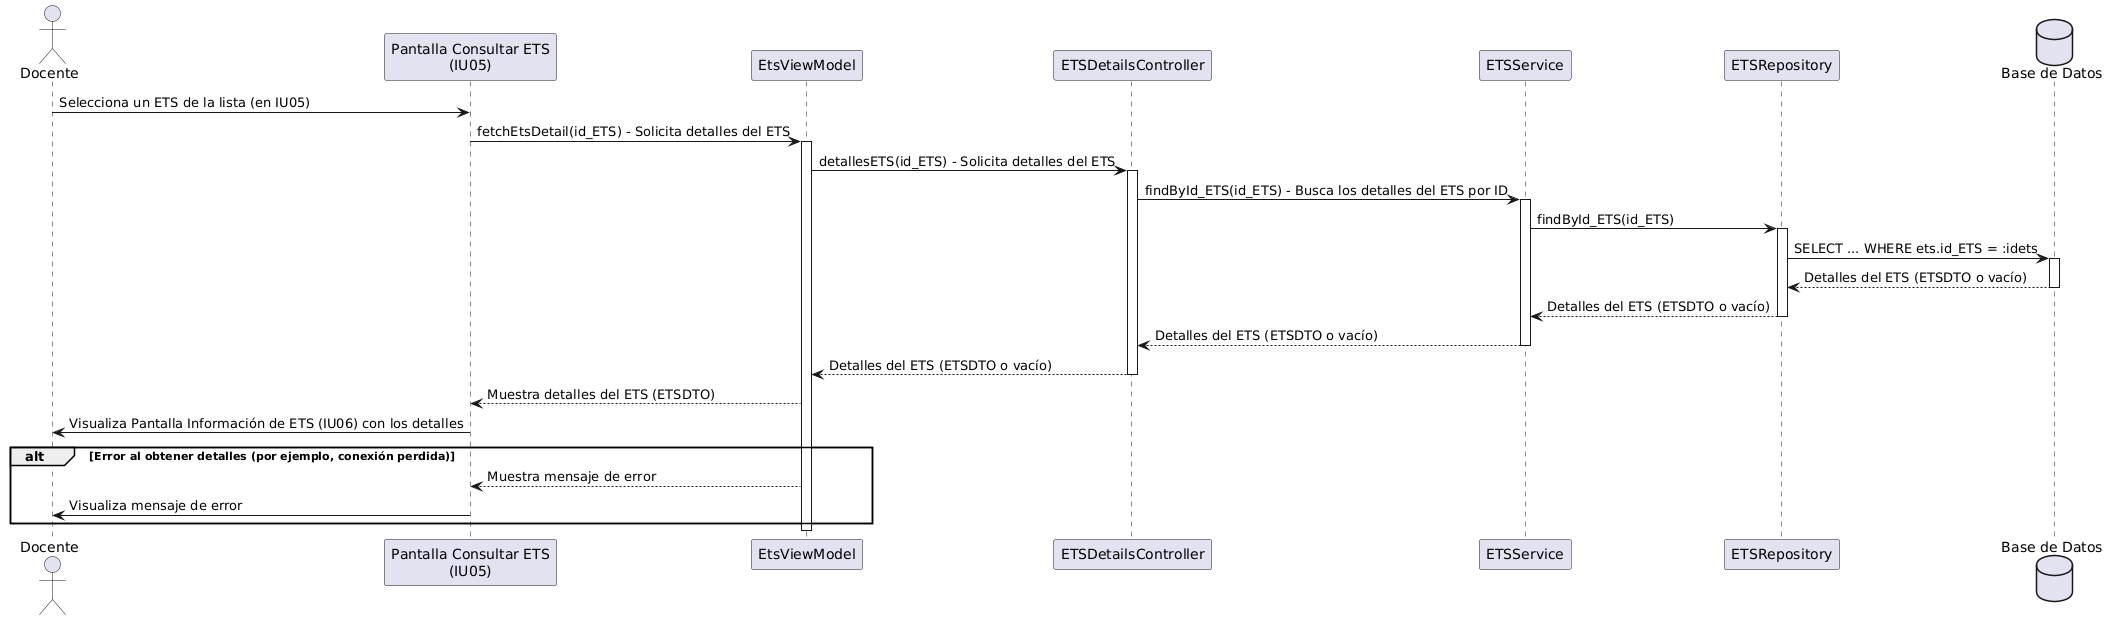
\includegraphics[width=1\textwidth]{Secuencia/CU-06.png}}
		\caption{Diagrama de secuencia del caso de uso número 06 (Mostrar información de los ETS asignados).}
		\label{fig:Diagrama de secuencia CU-06}
	\end{center}
\end{figure}

En el diagrama de secuencia \ref{fig:Diagrama de secuencia CU-06} se describe el proceso planeado para el caso de uso \hyperlink{CU-06}{CU-06 Mostrar información de los ETS asignados}, mostrando las interacciones que tendrá con la vista, el controlador, el servicio, el repositorio y la base de datos.

\newpage

\subsection{SE-07 Solicitar remplazo}

\begin{figure}[htbp!]
	\begin{center}
		\fbox{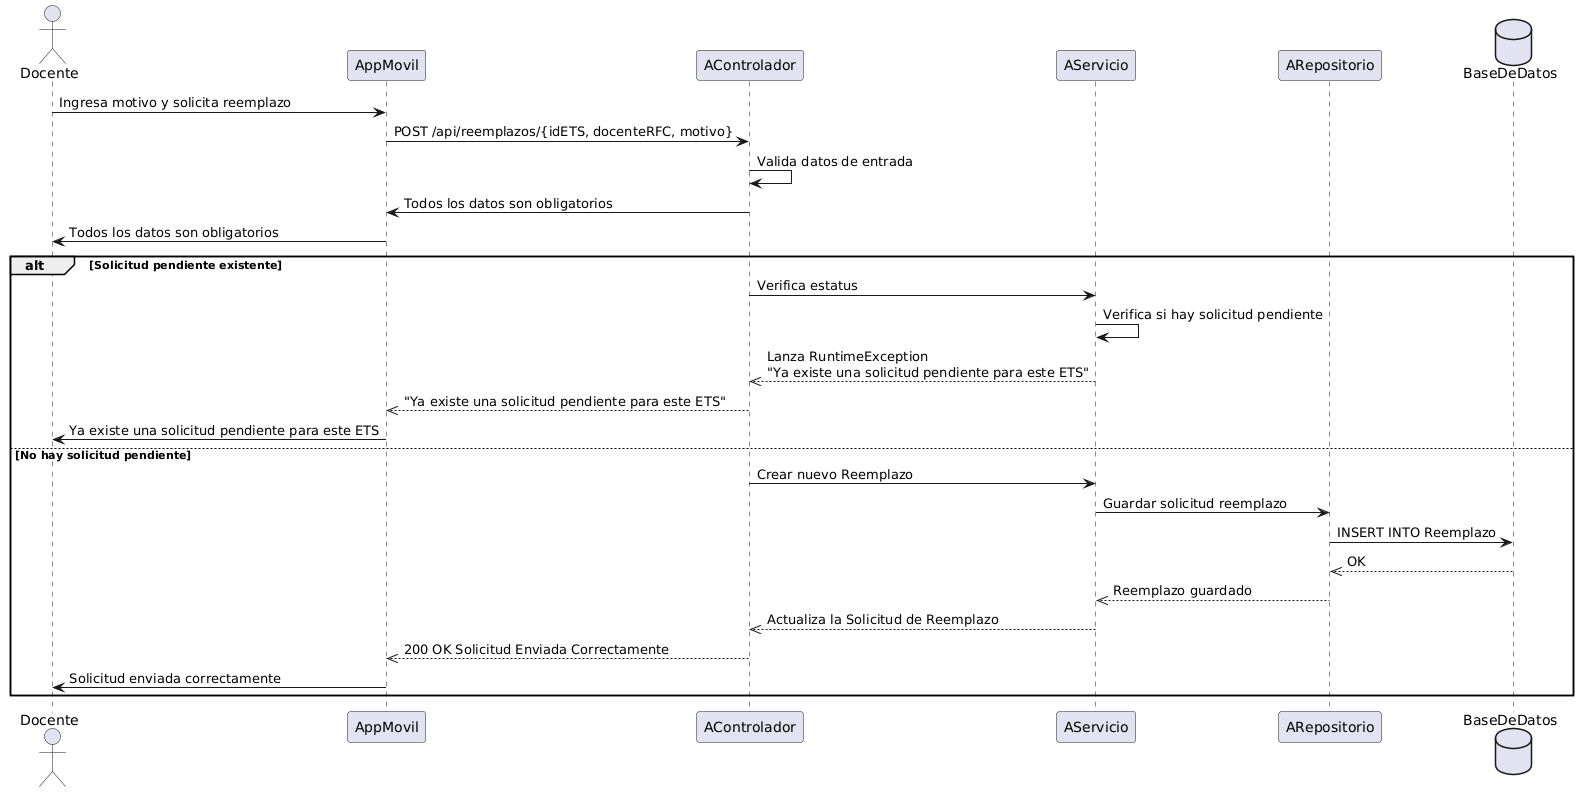
\includegraphics[width=1\textwidth]{Secuencia/CU-07.png}}
		\caption{Diagrama de secuencia del caso de uso número 07 (Solicitar remplazo).}
		\label{fig:Diagrama de secuencia CU-07}
	\end{center}
\end{figure}

En el diagrama de secuencia \ref{fig:Diagrama de secuencia CU-07} se describe el proceso planeado para el caso de uso \hyperlink{CU-07}{CU-07 Solicitar remplazo}, mostrando las interacciones que tendrá con la vista, el controlador, el servicio, el repositorio y la base de datos.

\newpage

\subsection{SE-08 Consultar lista de alumnos inscritos a un ETS}

\begin{figure}[htbp!]
	\begin{center}
		\fbox{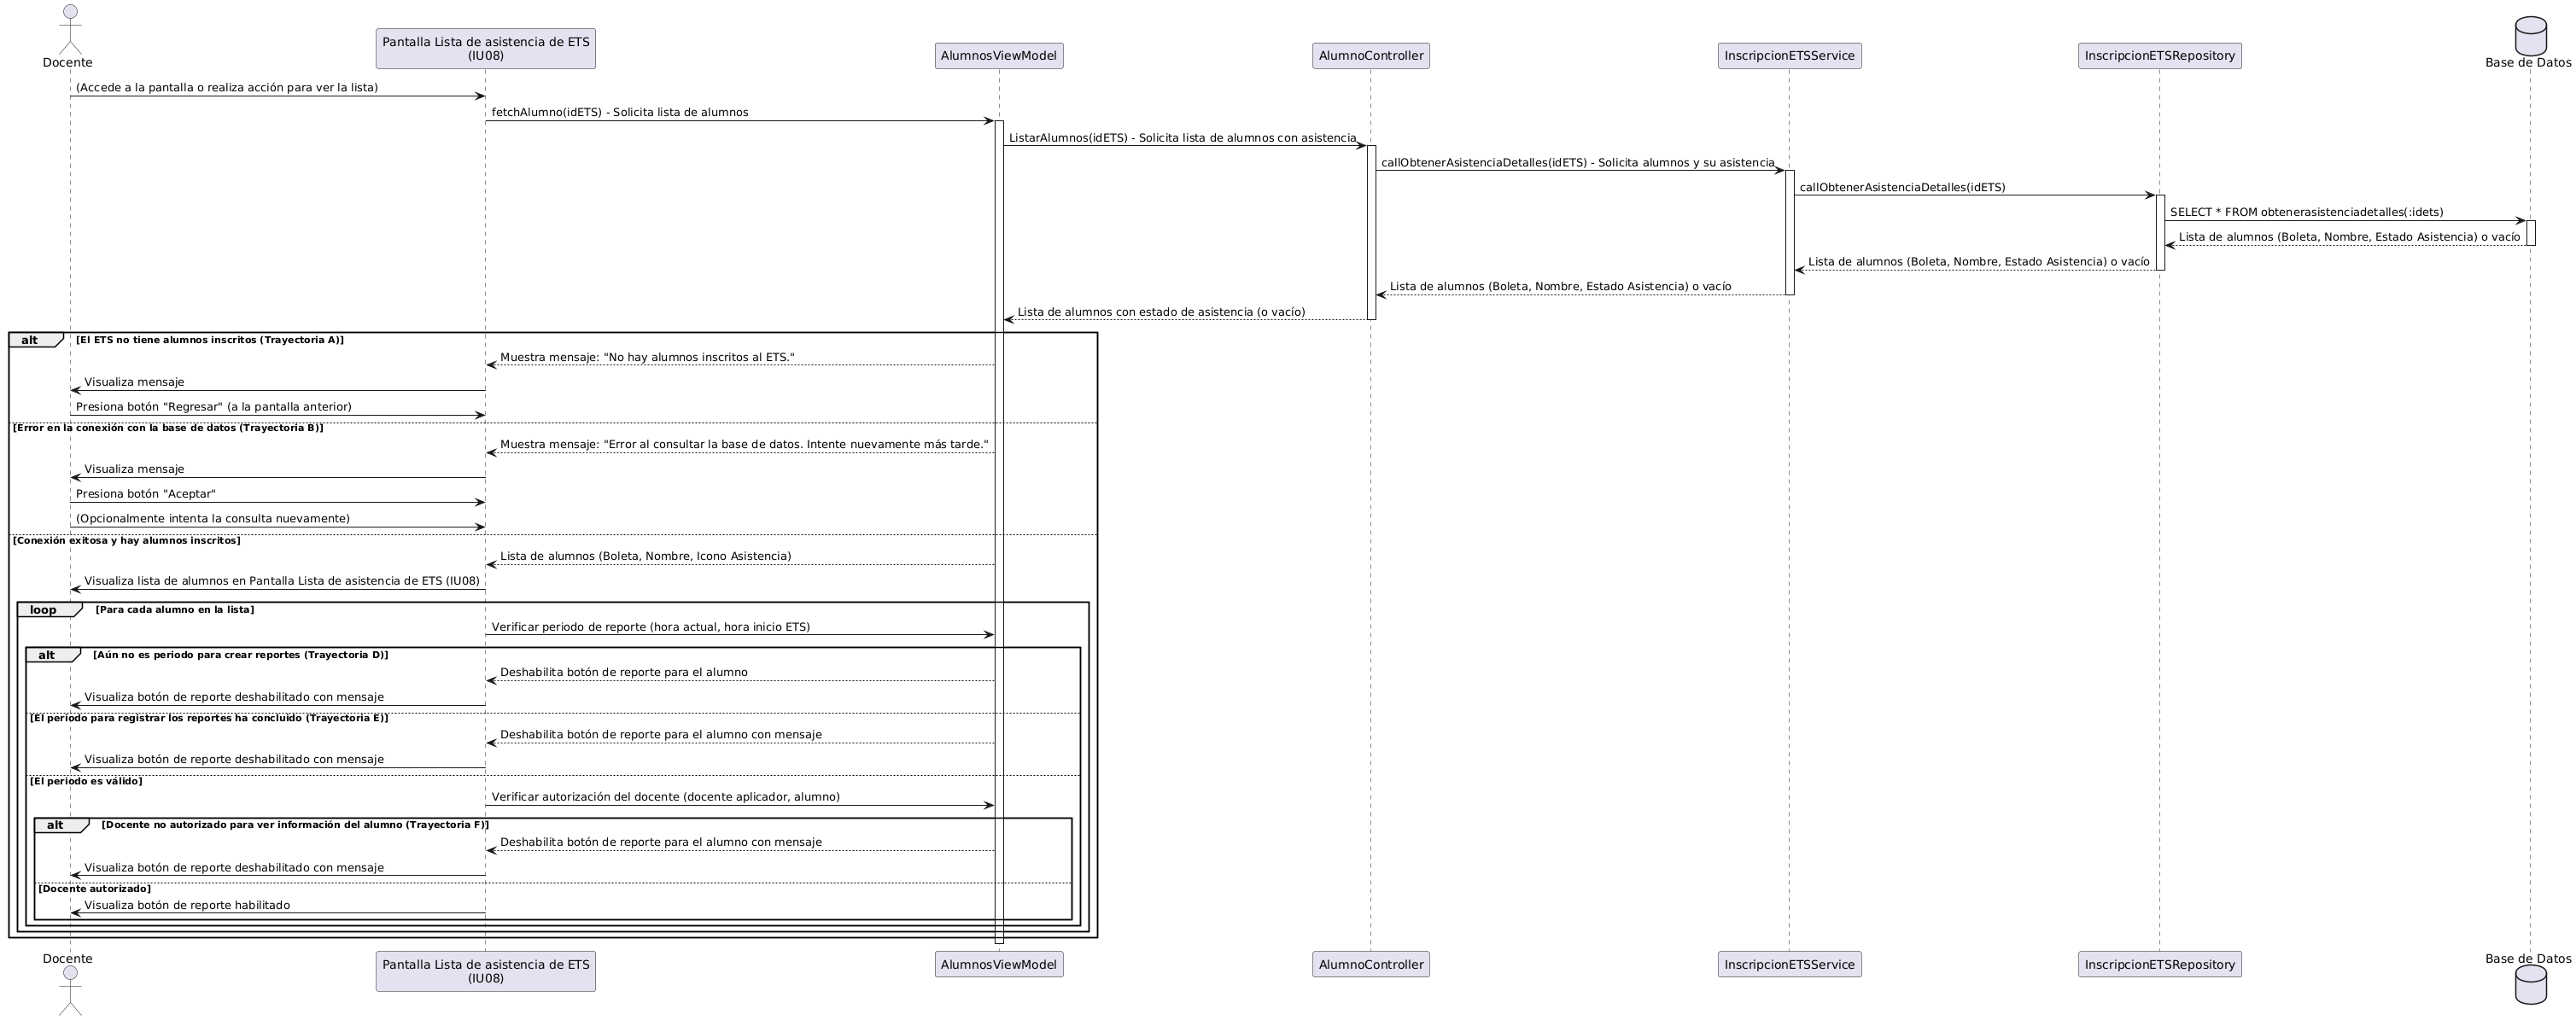
\includegraphics[width=1\textwidth]{Secuencia/CU-08.png}}
		\caption{Diagrama de secuencia del caso de uso número 08 (Consultar lista de alumnos inscritos a un ETS).}
		\label{fig:Diagrama de secuencia CU-08}
	\end{center}
\end{figure}

En el diagrama de secuencia \ref{fig:Diagrama de secuencia CU-08} se describe el proceso planeado para el caso de uso \hyperlink{CU-08}{CU-08 Consultar lista de alumnos inscritos a un ETS}, mostrando las interacciones que tendrá con la vista, el controlador, el servicio, el repositorio y la base de datos.

\newpage

\subsection{SE-09 Tomar asistencias a los ETS}

\begin{figure}[htbp!]
	\begin{center}
		\fbox{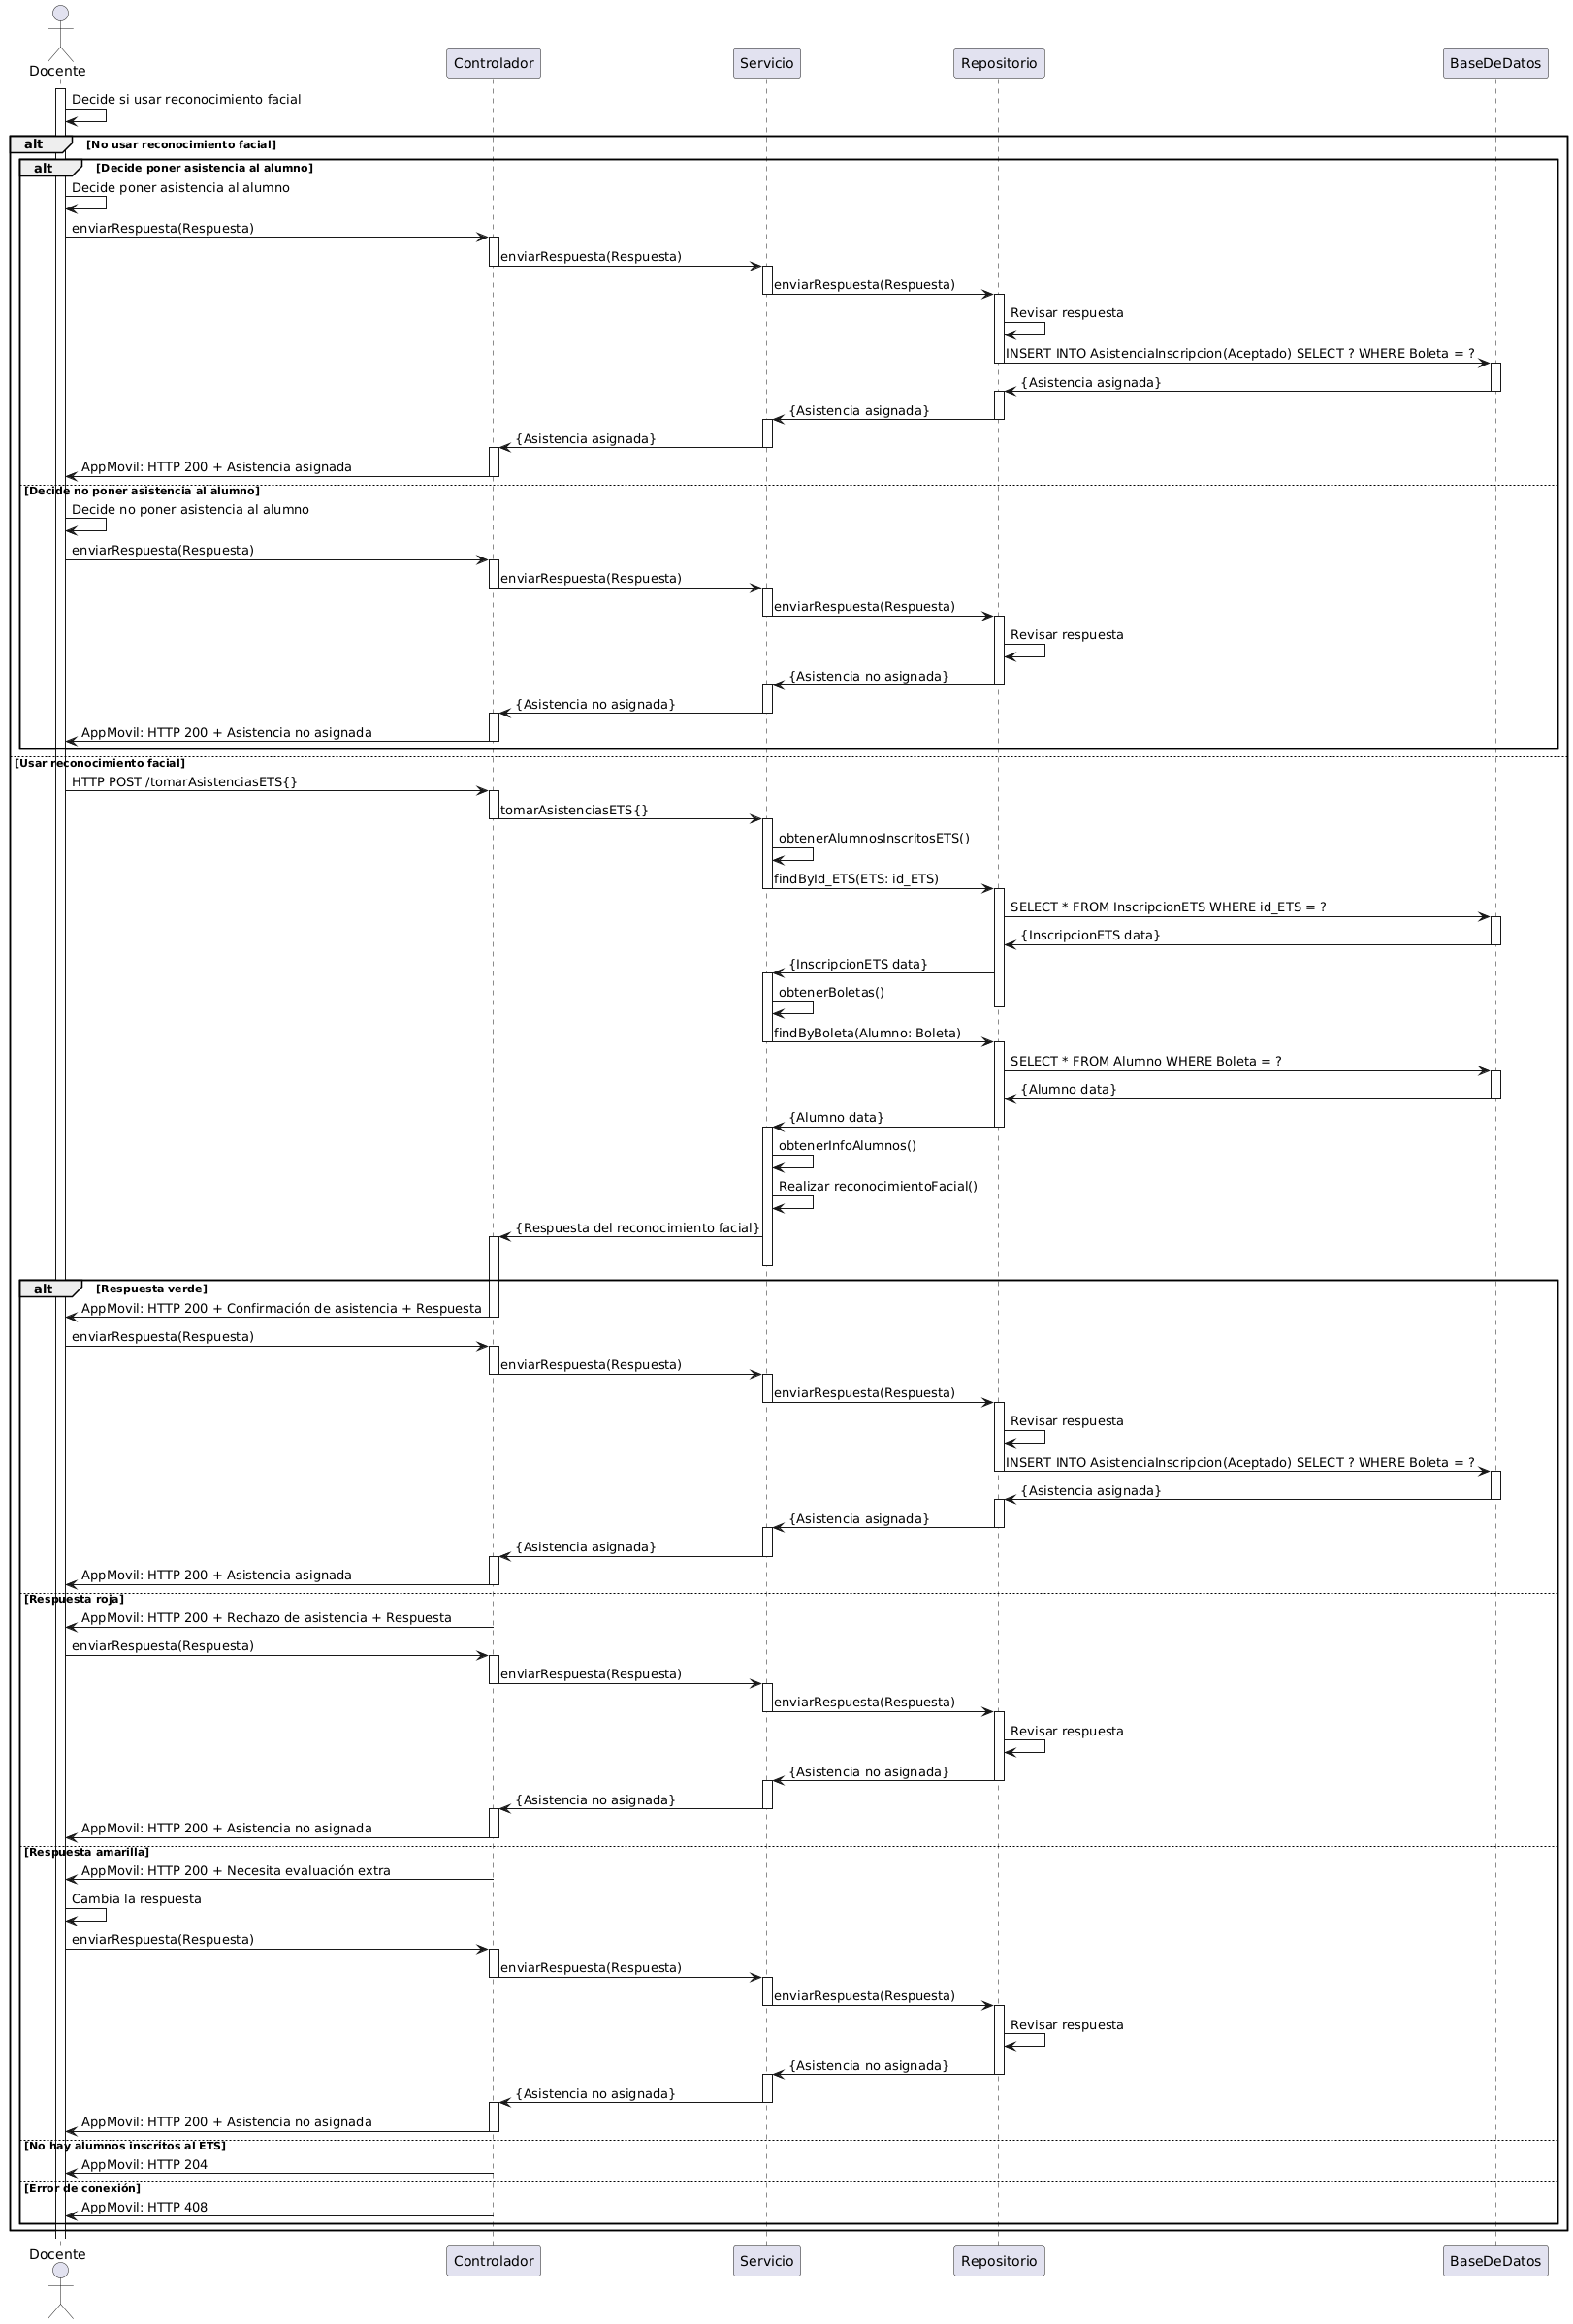
\includegraphics[width=.7\textwidth]{Secuencia/CU-09.png}}
		\caption{Diagrama de secuencia del caso de uso número 09 (Tomar asistencias a los ETS).}
		\label{fig:Diagrama de secuencia CU-09}
	\end{center}
\end{figure}

En el diagrama de secuencia \ref{fig:Diagrama de secuencia CU-09} se describe el proceso planeado para el caso de uso \hyperlink{CU-09}{CU-09 Tomar asistencias a los ETS}, mostrando las interacciones que tendrá con la vista, el controlador, el servicio, el repositorio y la base de datos.

\subsection{SE-10 Consultar lista de asistencia de alumnos inscritos a los ETS}

\begin{figure}[htbp!]
	\begin{center}
		\fbox{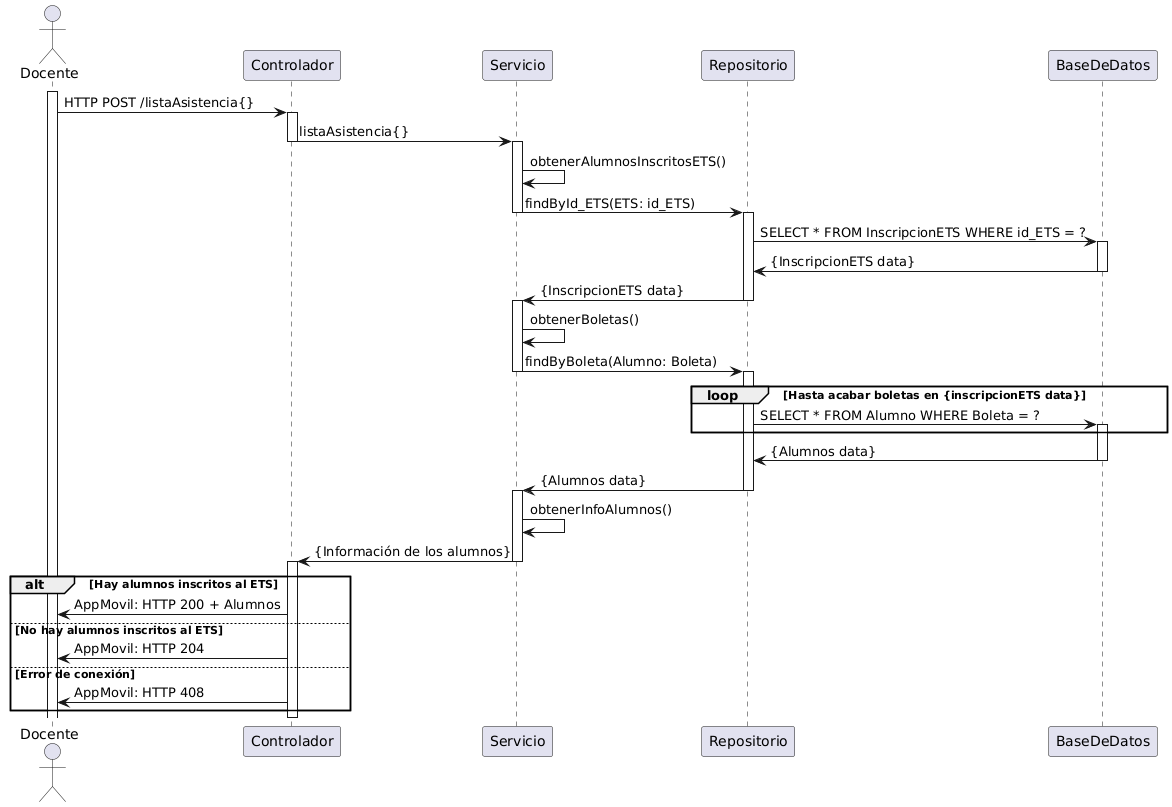
\includegraphics[width=1\textwidth]{Secuencia/CU-10.png}}
		\caption{Diagrama de secuencia del caso de uso número 10 (Consultar lista de asistencia de alumnos inscritos a los ETS).}
		\label{fig:Diagrama de secuencia CU-10}
	\end{center}
\end{figure}

En el diagrama de secuencia \ref{fig:Diagrama de secuencia CU-10} se describe el proceso planeado para el caso de uso \hyperlink{CU-10}{CU-10 Consultar lista de asistencia de alumnos inscritos a los ETS}, mostrando las interacciones que tendrá con la vista, el controlador, el servicio, el repositorio y la base de datos.

\newpage

\subsection{SE-11 Mostrar la foto e información  del alumno}

\begin{figure}[htbp!]
	\begin{center}
		\fbox{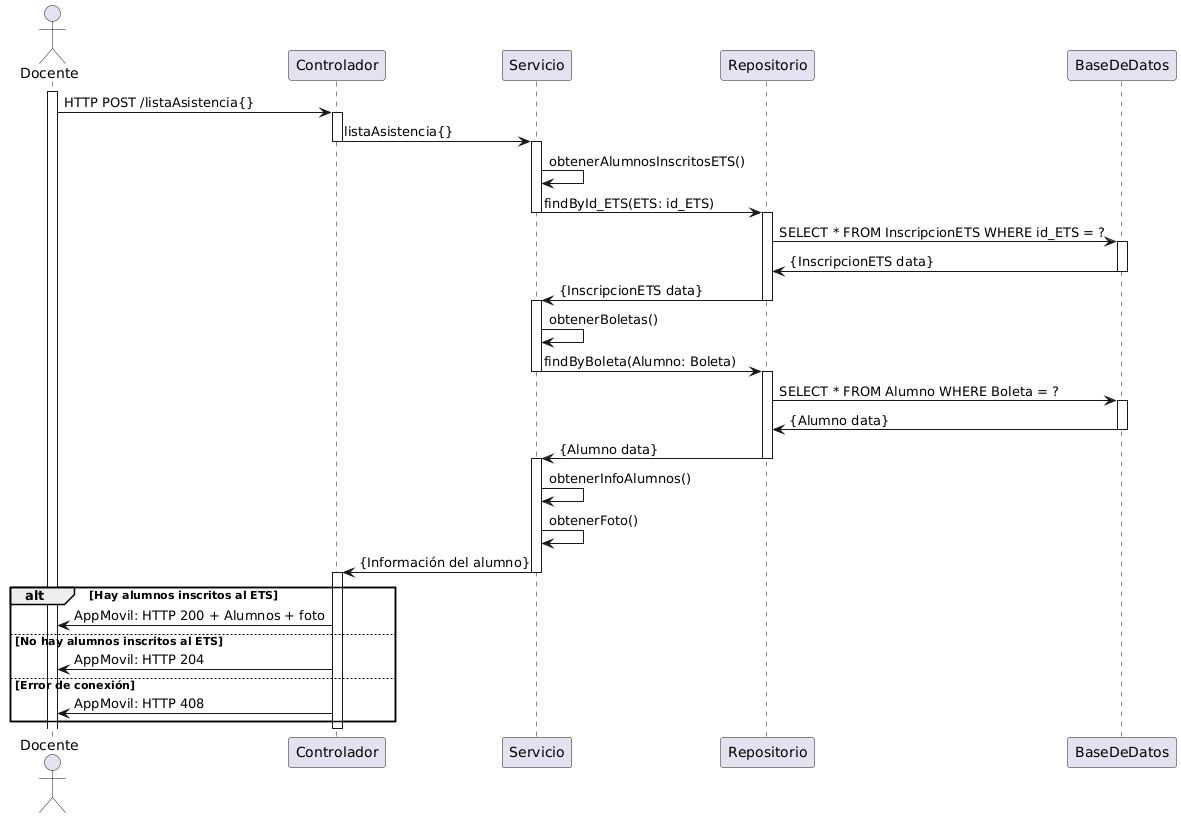
\includegraphics[width=1\textwidth]{Secuencia/CU-11.png}}
		\caption{Diagrama de secuencia del caso de uso número 11 (Mostrar la foto e información  del alumno).}
		\label{fig:Diagrama de secuencia CU-11}
	\end{center}
\end{figure}


En el diagrama de secuencia \ref{fig:Diagrama de secuencia CU-11} se describe el proceso planeado para el caso de uso \hyperlink{CU-11}{CU-11 Mostrar la foto e información  del alumno}, mostrando las interacciones que tendrá con la vista, el controlador, el servicio, el repositorio y la base de datos.

\newpage

\subsection{SE-12 Consultar alumno mediante código QR de la credencial}

\begin{figure}[htbp!]
	\begin{center}
		\fbox{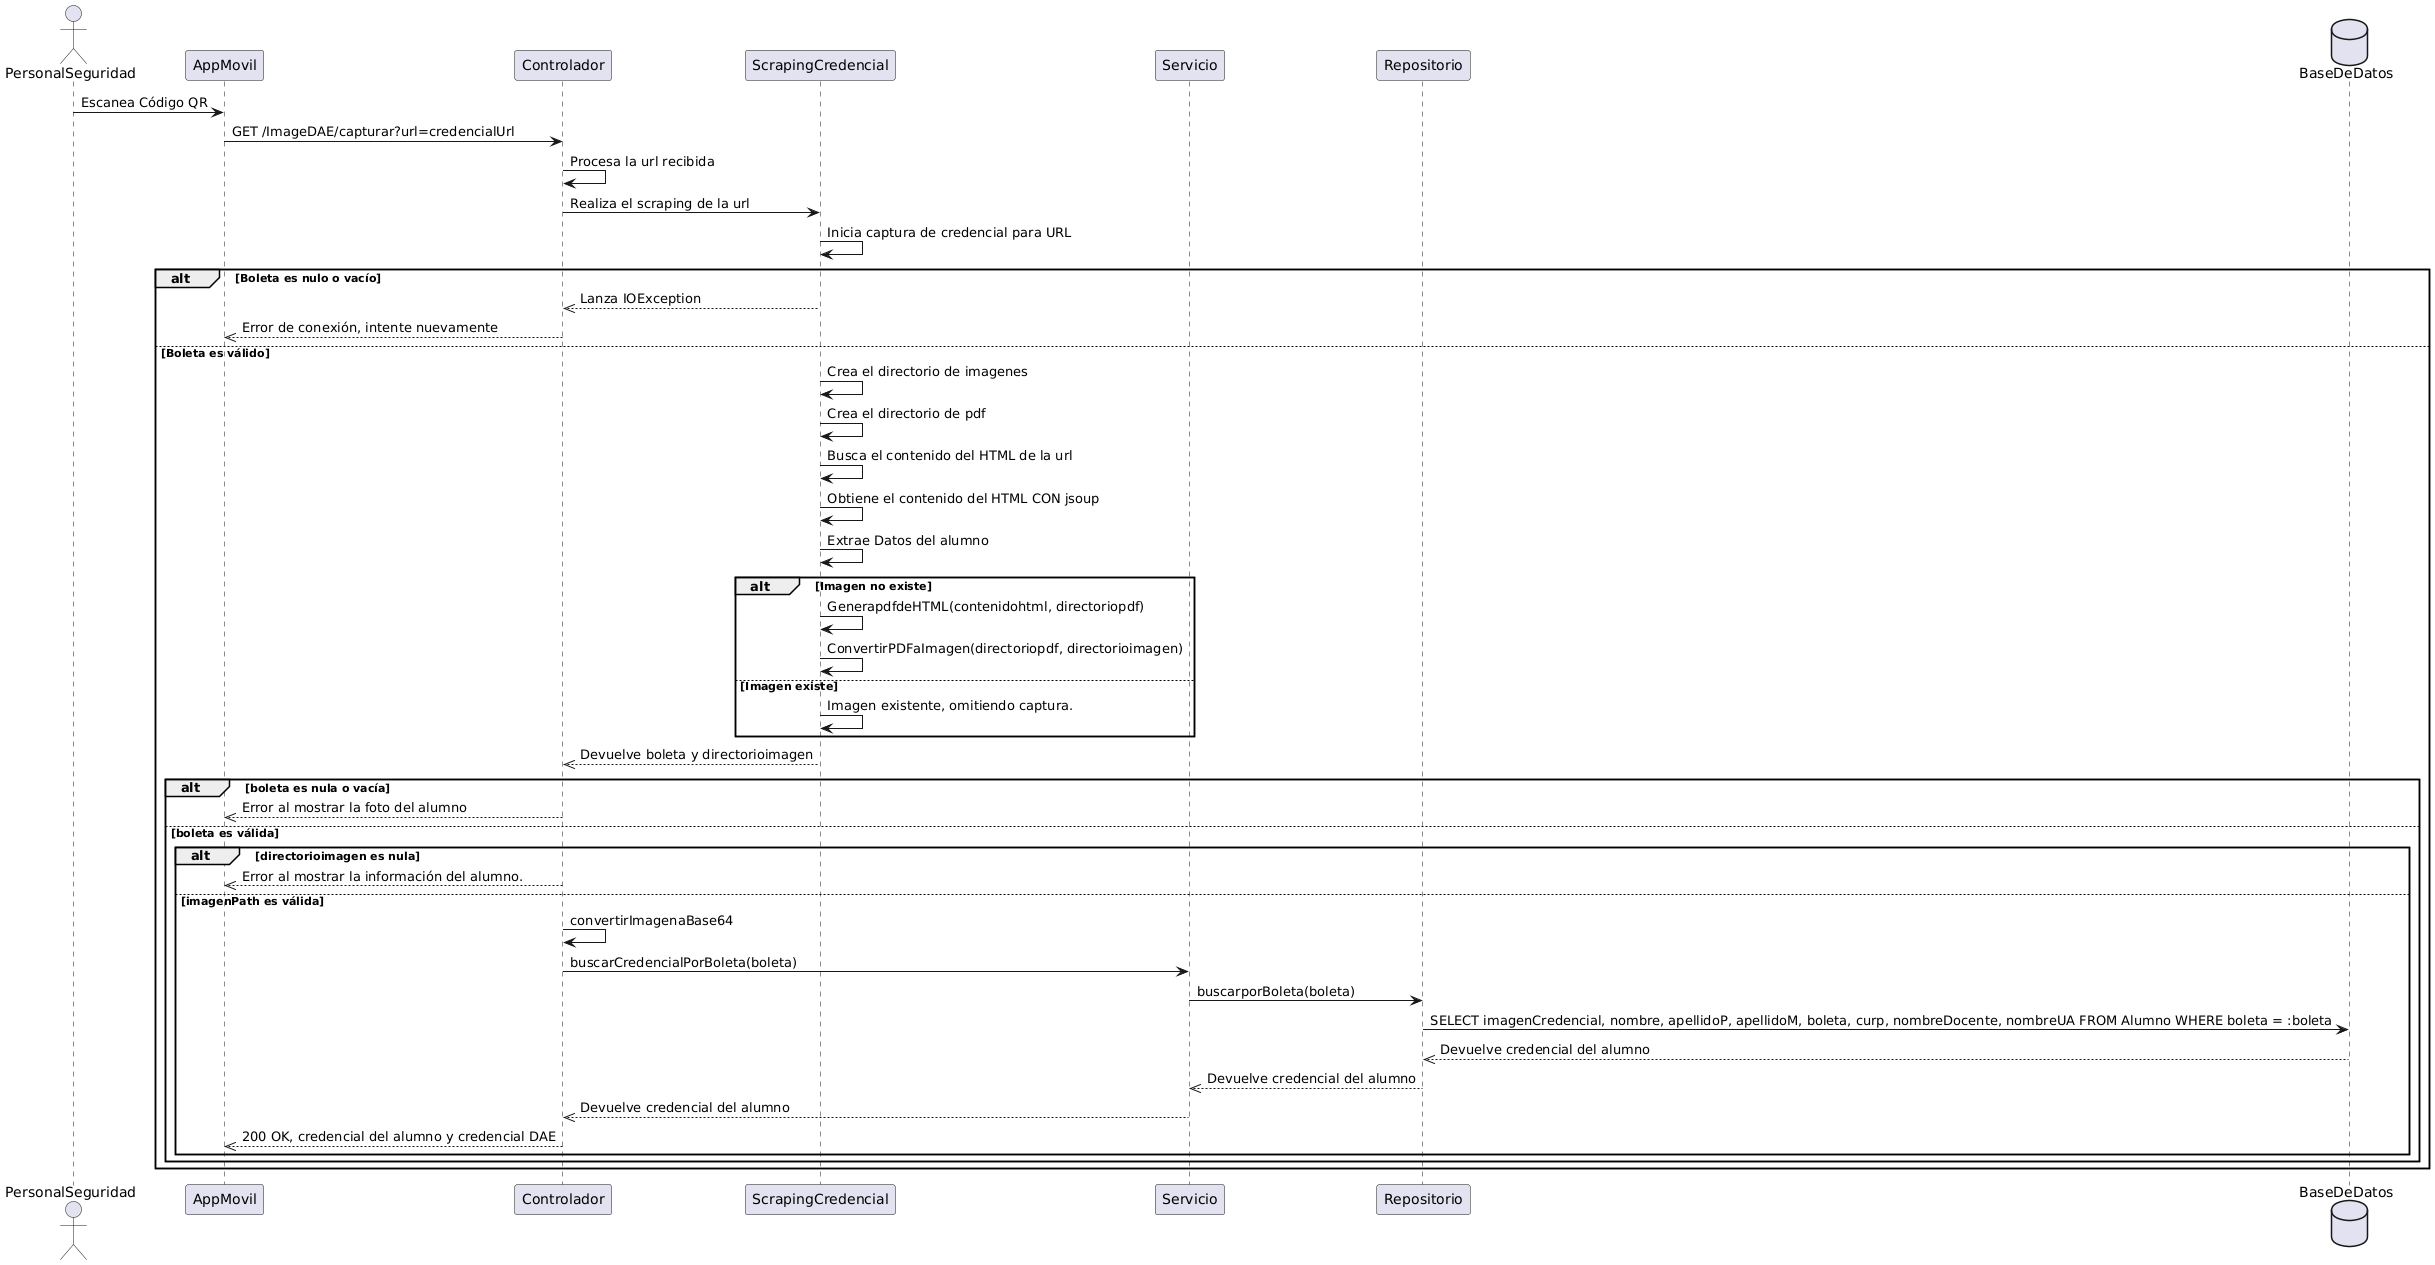
\includegraphics[width=1\textwidth]{Secuencia/CU-12.png}}
		\caption{Diagrama de secuencia del caso de uso número 12 (Consultar alumno mediante código QR de la credencial).}
		\label{fig:Diagrama de secuencia CU-12}
	\end{center}
\end{figure}

En el diagrama de secuencia \ref{fig:Diagrama de secuencia CU-12} se describe el proceso planeado para el caso de uso \hyperlink{CU-12}{CU-12 Consultar alumno mediante código QR de la credencial}, mostrando las interacciones que tendrá con la vista, el controlador, el servicio, el repositorio y la base de datos.

\newpage

\subsection{SE-13 Buscar alumno por boleta}

\begin{figure}[htbp!]
	\begin{center}
		\fbox{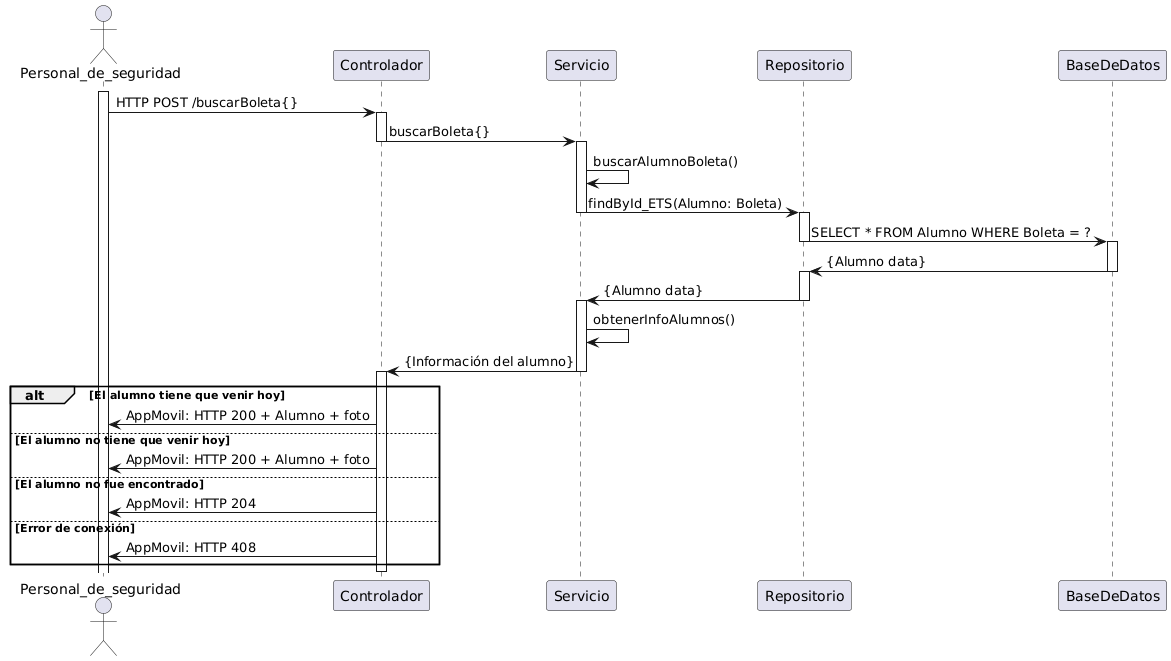
\includegraphics[width=1\textwidth]{Secuencia/CU-13.png}}
		\caption{Diagrama de secuencia del caso de uso número 13 (Buscar alumno por boleta).}
		\label{fig:Diagrama de secuencia CU-13}
	\end{center}
\end{figure}

En el diagrama de secuencia \ref{fig:Diagrama de secuencia CU-13} se describe el proceso planeado para el caso de uso \hyperlink{CU-13}{CU-13 Buscar alumno por boleta}, mostrando las interacciones que tendrá con la vista, el controlador, el servicio, el repositorio y la base de datos.

\newpage

\subsection{SE-14 Buscar alumno por nombre}

\begin{figure}[htbp!]
	\begin{center}
		\fbox{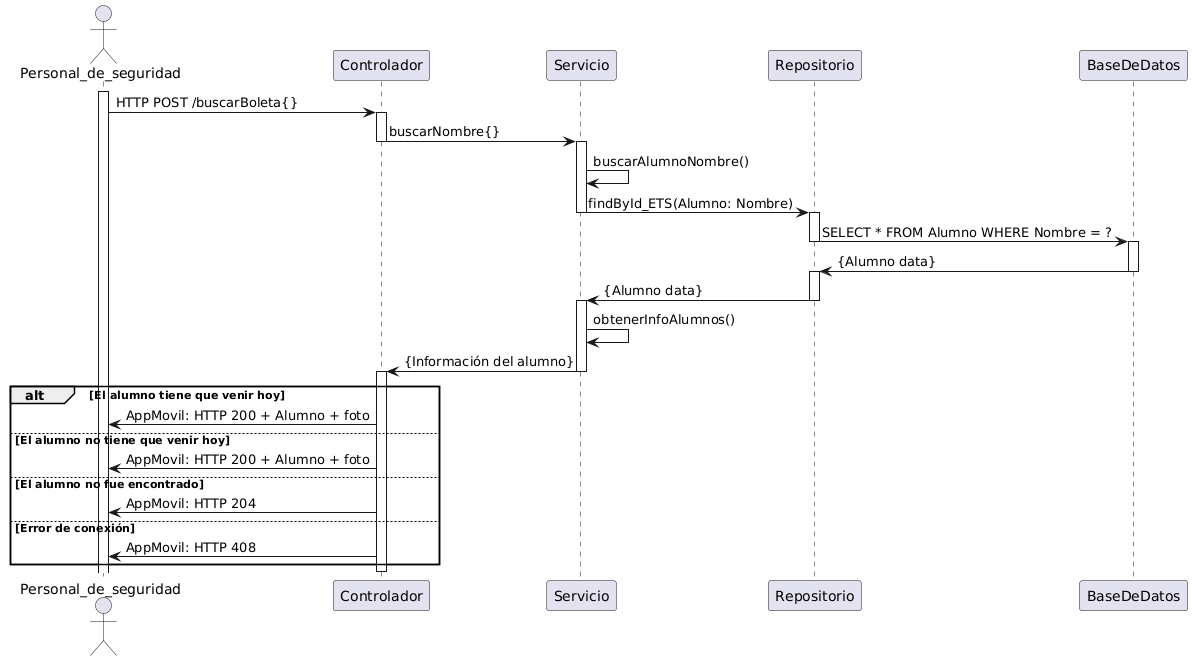
\includegraphics[width=1\textwidth]{Secuencia/CU-14.png}}
		\caption{Diagrama de secuencia del caso de uso número 14 (Buscar alumno por nombre).}
		\label{fig:Diagrama de secuencia CU-14}
	\end{center}
\end{figure}

En el diagrama de secuencia \ref{fig:Diagrama de secuencia CU-14} se describe el proceso planeado para el caso de uso \hyperlink{CU-14}{CU-14 Buscar alumno por nombre}, mostrando las interacciones que tendrá con la vista, el controlador, el servicio, el repositorio y la base de datos.

\newpage

\subsection{SE-15 Registrar asistencia}

\begin{figure}[htbp!]
	\begin{center}
		\fbox{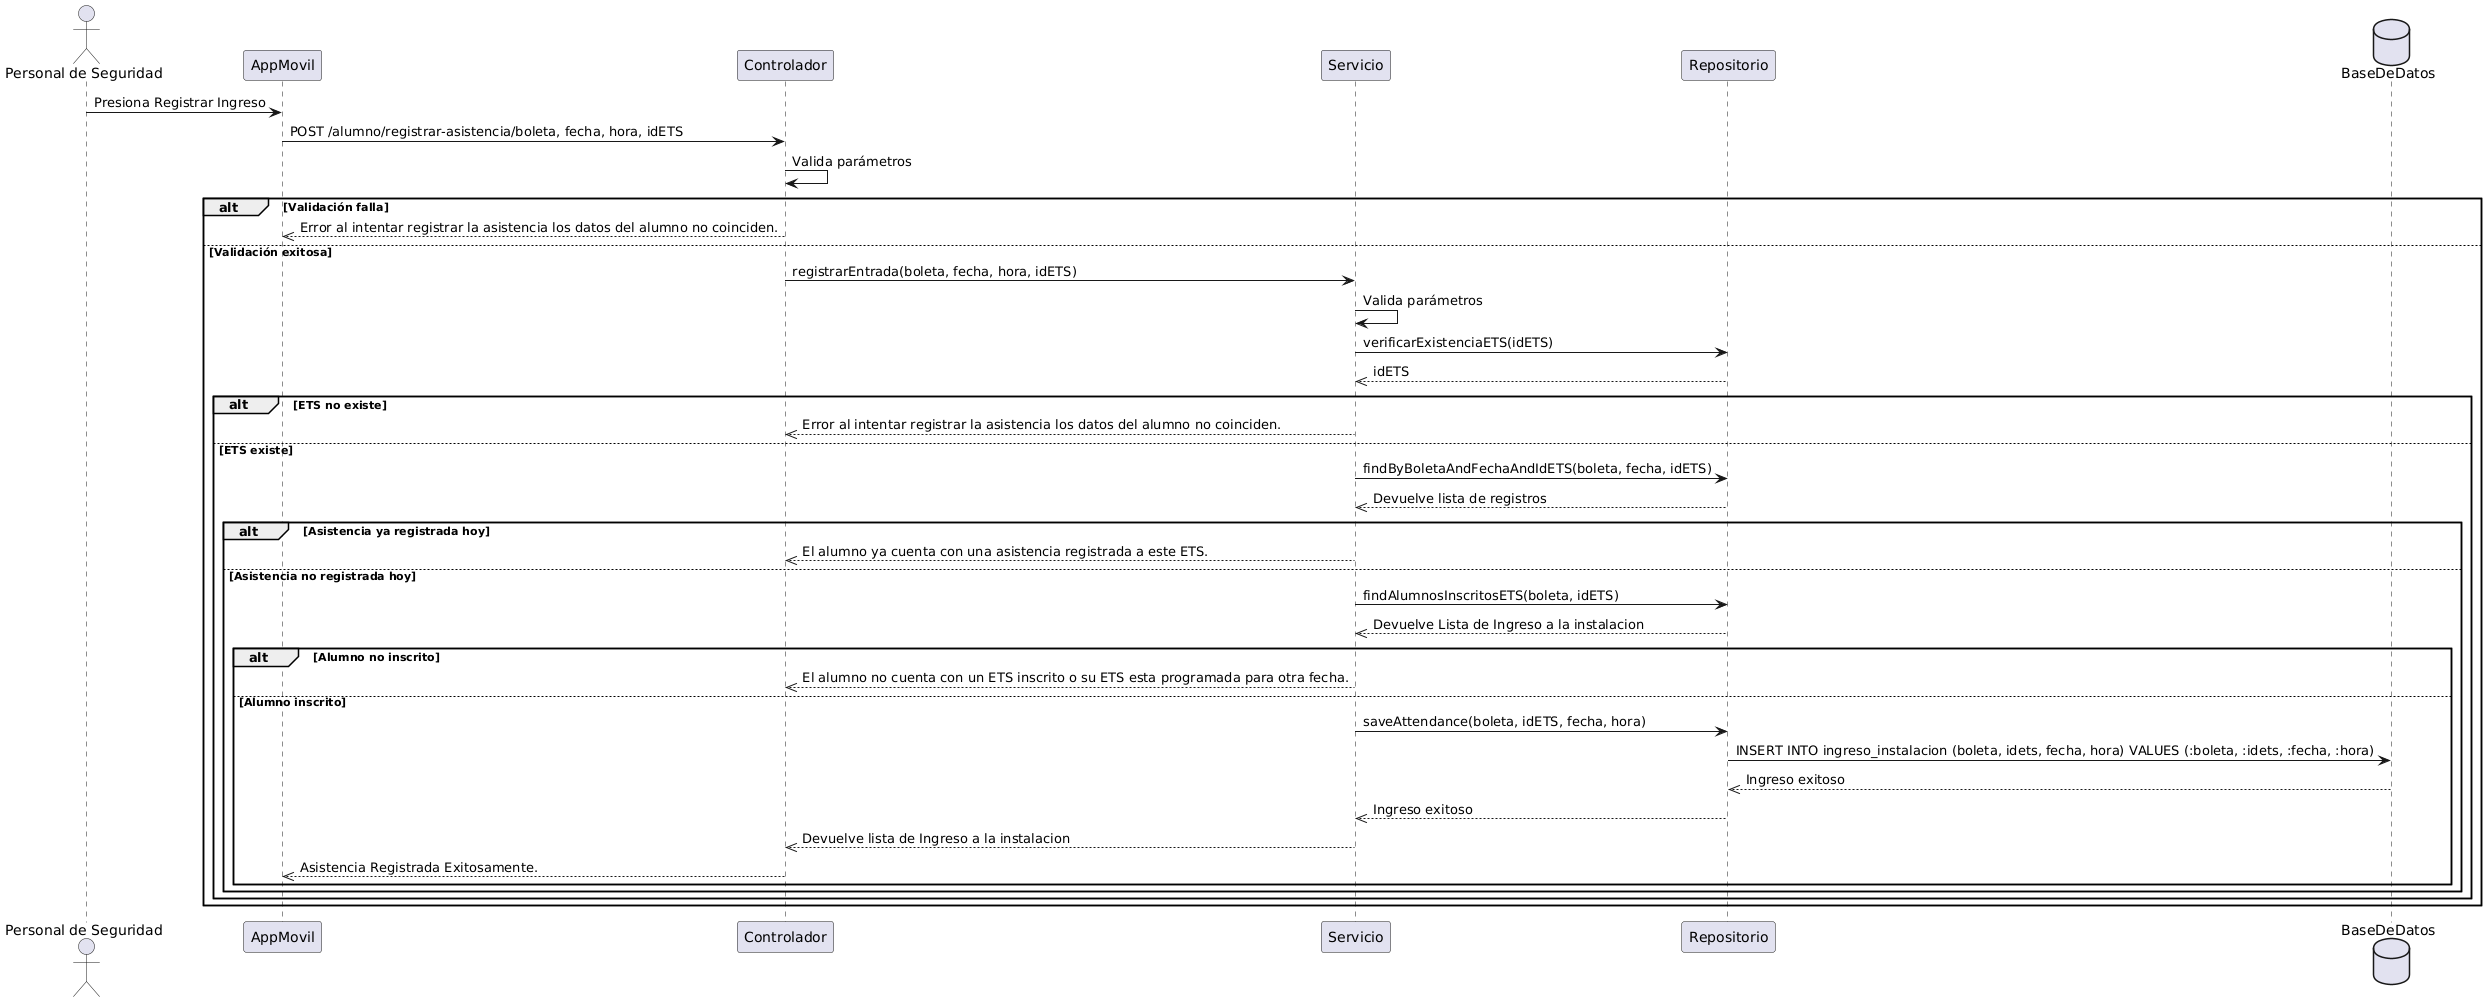
\includegraphics[width=.7\textwidth]{Secuencia/CU-15.png}}
		\caption{Diagrama de secuencia del caso de uso número 15 (Registrar asistencia).}
		\label{fig:Diagrama de secuencia CU-15}
	\end{center}
\end{figure}

En el diagrama de secuencia \ref{fig:Diagrama de secuencia CU-15} se describe el proceso planeado para el caso de uso \hyperlink{CU-15}{CU-15 Registrar asistencia}, mostrando las interacciones que tendrá con la vista, el controlador, el servicio, el repositorio y la base de datos.

\subsection{SE-16 Consultar periodos de ETS inscritos del alumno}

\begin{figure}[htbp!]
	\begin{center}
		\fbox{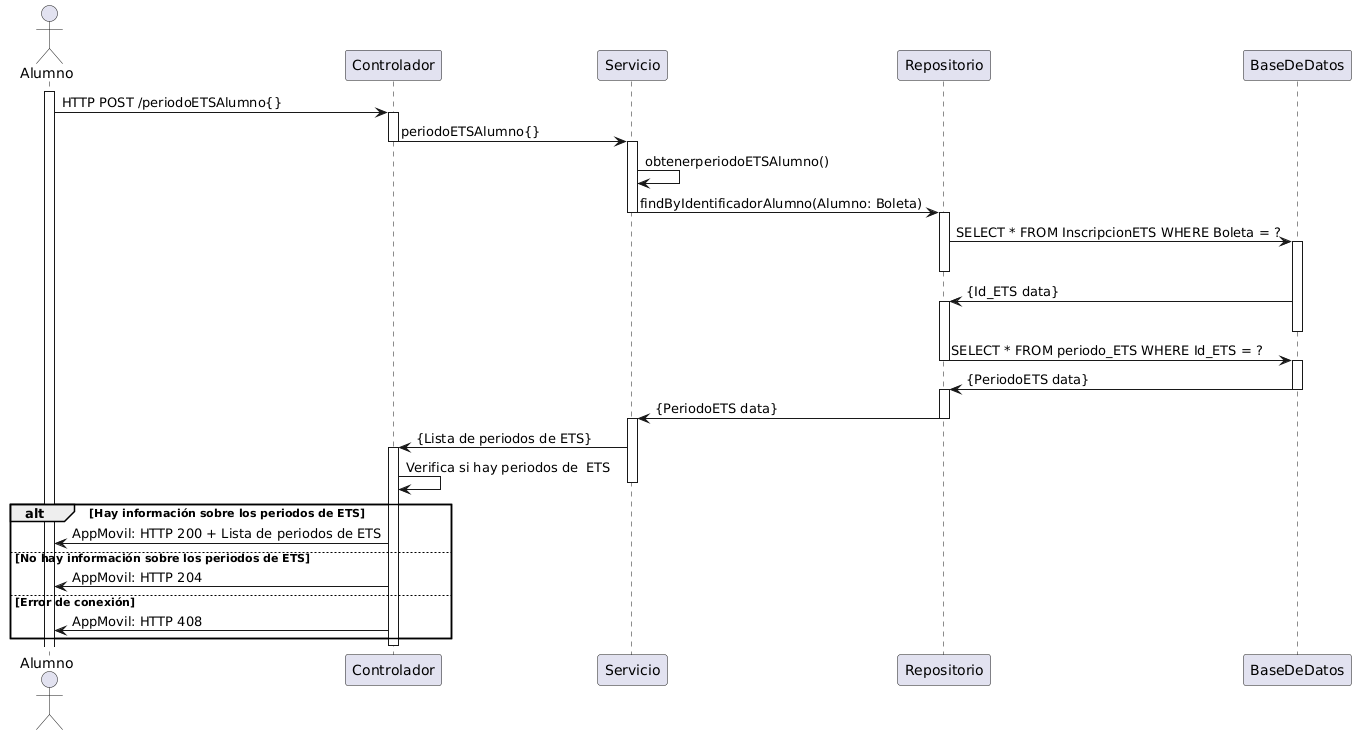
\includegraphics[width=1\textwidth]{Secuencia/CU-16.png}}
		\caption{Diagrama de secuencia del caso de uso número 16 (Consultar periodos de ETS inscritos del alumno).}
		\label{fig:Diagrama de secuencia CU-16}
	\end{center}
\end{figure}

En el diagrama de secuencia \ref{fig:Diagrama de secuencia CU-16} se describe el proceso planeado para el caso de uso \hyperlink{CU-16}{CU-16 Consultar periodos de ETS inscritos del alumno}, mostrando las interacciones que tendrá con la vista, el controlador, el servicio, el repositorio y la base de datos.

\newpage

\subsection{SE-17 Consultar ETS inscritos}

\begin{figure}[htbp!]
	\begin{center}
		\fbox{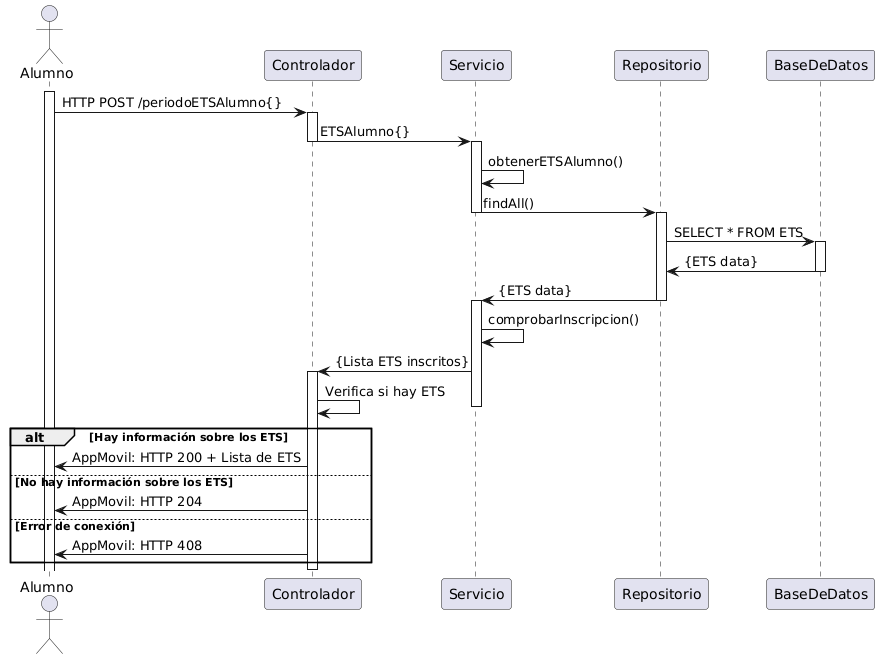
\includegraphics[width=1\textwidth]{Secuencia/CU-17.png}}
		\caption{Diagrama de secuencia del caso de uso número 04 (Consultar ETS inscritos).}
		\label{fig:Diagrama de secuencia CU-17}
	\end{center}
\end{figure}

En el diagrama de secuencia \ref{fig:Diagrama de secuencia CU-17} se describe el proceso planeado para el caso de uso \hyperlink{CU-17}{CU-17 Consultar  ETS inscritos}, mostrando las interacciones que tendrá con la vista, el controlador, el servicio, el repositorio y la base de datos.

\newpage

\subsection{SE-18 Mostrar información del los ETS inscritos}

\begin{figure}[htbp!]
	\begin{center}
		\fbox{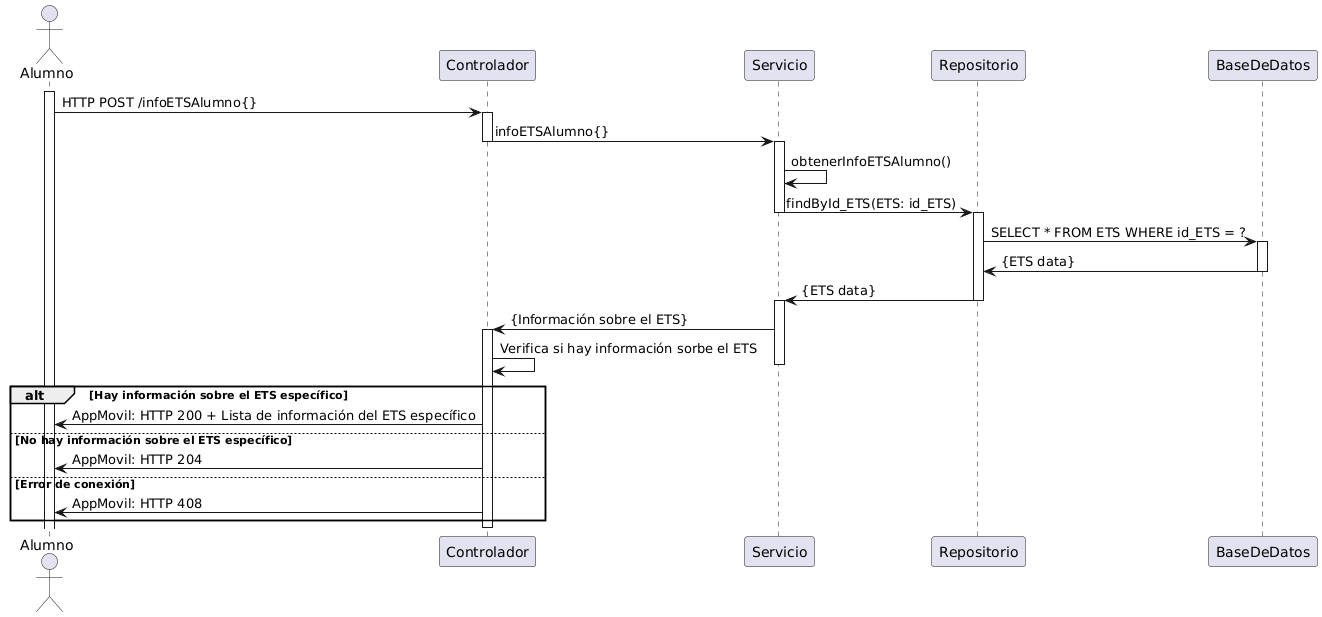
\includegraphics[width=1\textwidth]{Secuencia/CU-18.png}}
		\caption{Diagrama de secuencia del caso de uso número 18 (Mostrar información del los ETS inscritos).}
		\label{fig:Diagrama de secuencia CU-18}
	\end{center}
\end{figure}

En el diagrama de secuencia \ref{fig:Diagrama de secuencia CU-18} se describe el proceso planeado para el caso de uso \hyperlink{CU-18}{CU-18 Mostrar información del los ETS inscritos}, mostrando las interacciones que tendrá con la vista, el controlador, el servicio, el repositorio y la base de datos.

\newpage

\subsection{SE-19 Probar reconocimiento facial}

\begin{figure}[htbp!]
	\begin{center}
		\fbox{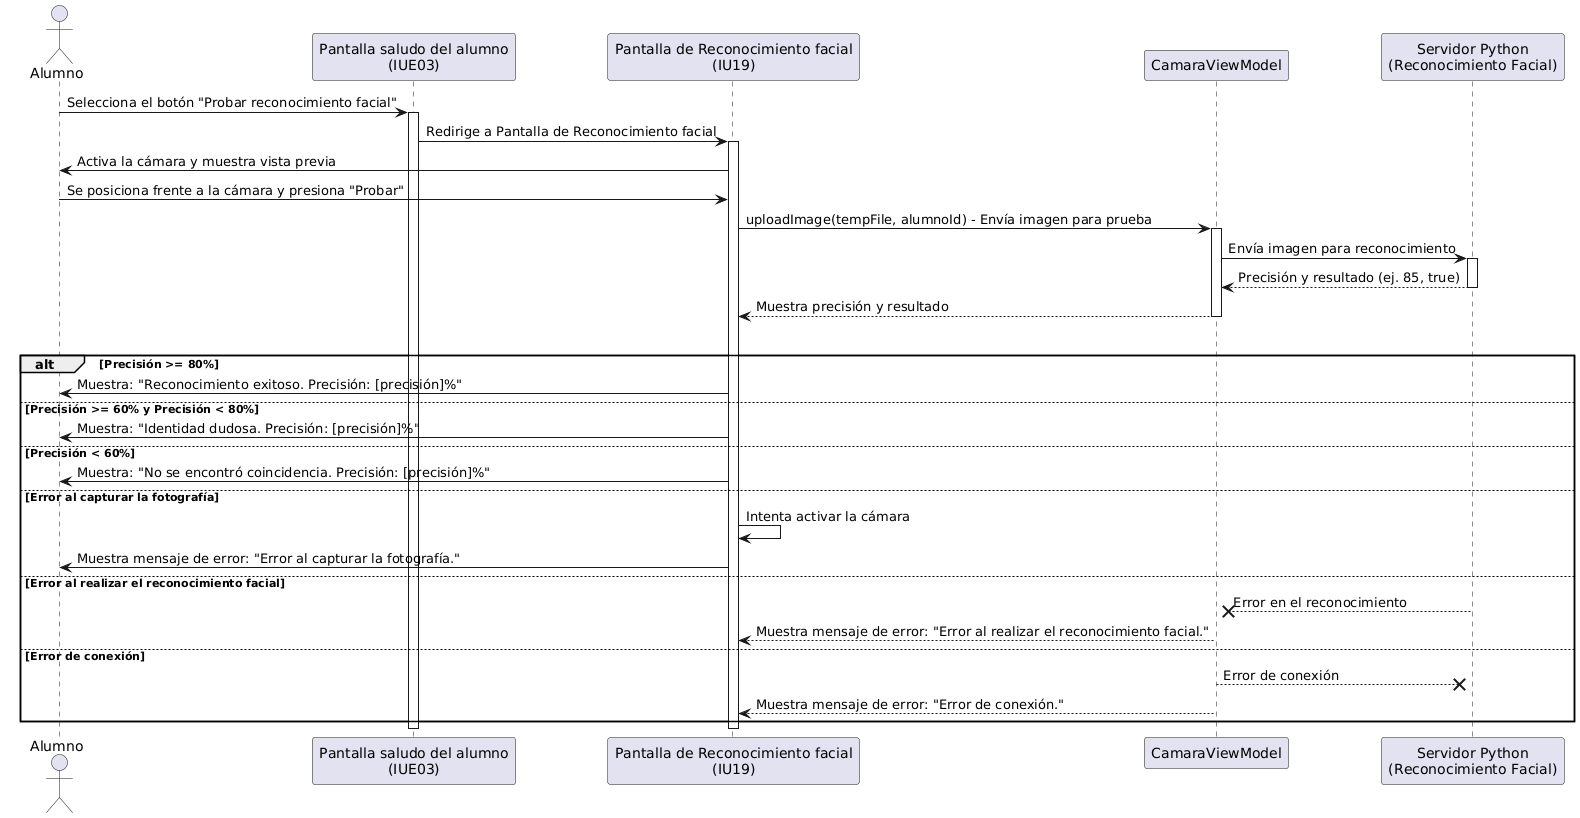
\includegraphics[width=1\textwidth]{Secuencia/CU-19.png}}
		\caption{Diagrama de secuencia del caso de uso número 19 (Probar reconocimiento facial).}
		\label{fig:Diagrama de secuencia CU-19}
	\end{center}
\end{figure}

En el diagrama de secuencia \ref{fig:Diagrama de secuencia CU-19} se describe el proceso planeado para el caso de uso \hyperlink{CU-19}{CU-19 Probar reconocimiento facial}, mostrando las interacciones que tendrá con la vista, el controlador, el servicio, el repositorio y la base de datos.

\newpage

\subsection{SE-20 Revisar información de acceso a los ETS}

\begin{figure}[htbp!]
	\begin{center}
		\fbox{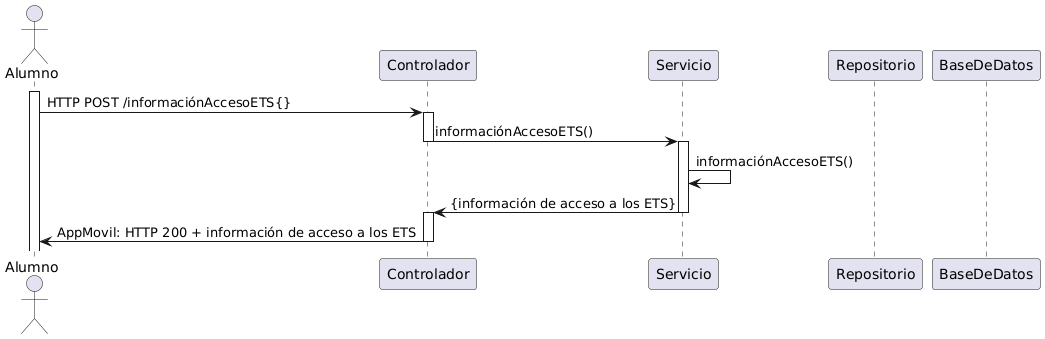
\includegraphics[width=1\textwidth]{Secuencia/CU-20.png}}
		\caption{Diagrama de secuencia del caso de uso número 20 (Revisar información de acceso a los ETS).}
		\label{fig:Diagrama de secuencia CU-20}
	\end{center}
\end{figure}

En el diagrama de secuencia \ref{fig:Diagrama de secuencia CU-20} se describe el proceso planeado para el caso de uso \hyperlink{CU-20}{CU-20 Revisar información de acceso a los ETS}, mostrando las interacciones que tendrá con la vista, el controlador, el servicio, el repositorio y la base de datos.

\newpage

\subsection{SE-21 Dar de alta a alumno}

\begin{figure}[htbp!]
	\begin{center}
		\fbox{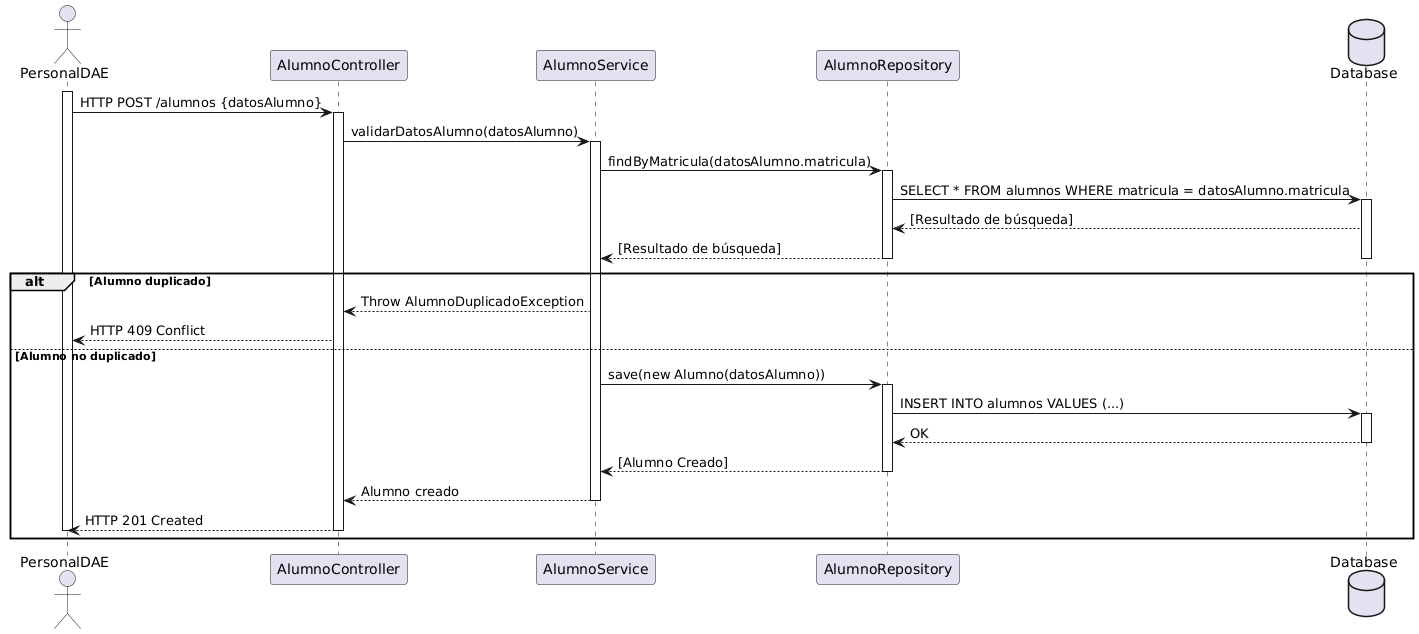
\includegraphics[width=1\textwidth]{Secuencia/CU-21.png}}
		\caption{Diagrama de secuencia del caso de uso número 21 (Dar de alta a alumno).}
		\label{fig:Diagrama de secuencia CU-21}
	\end{center}
\end{figure}

En el diagrama de secuencia \ref{fig:Diagrama de secuencia CU-21} se describe el proceso planeado para el caso de uso \hyperlink{CU-21}{CU-21 Dar de alta a alumno}, mostrando las interacciones que tendrá con la vista, el controlador, el servicio, el repositorio y la base de datos.

\newpage

\subsection{SE-22 Crear credencial y capturar fotografía estudiantil}

\begin{figure}[htbp!]
	\begin{center}
		\fbox{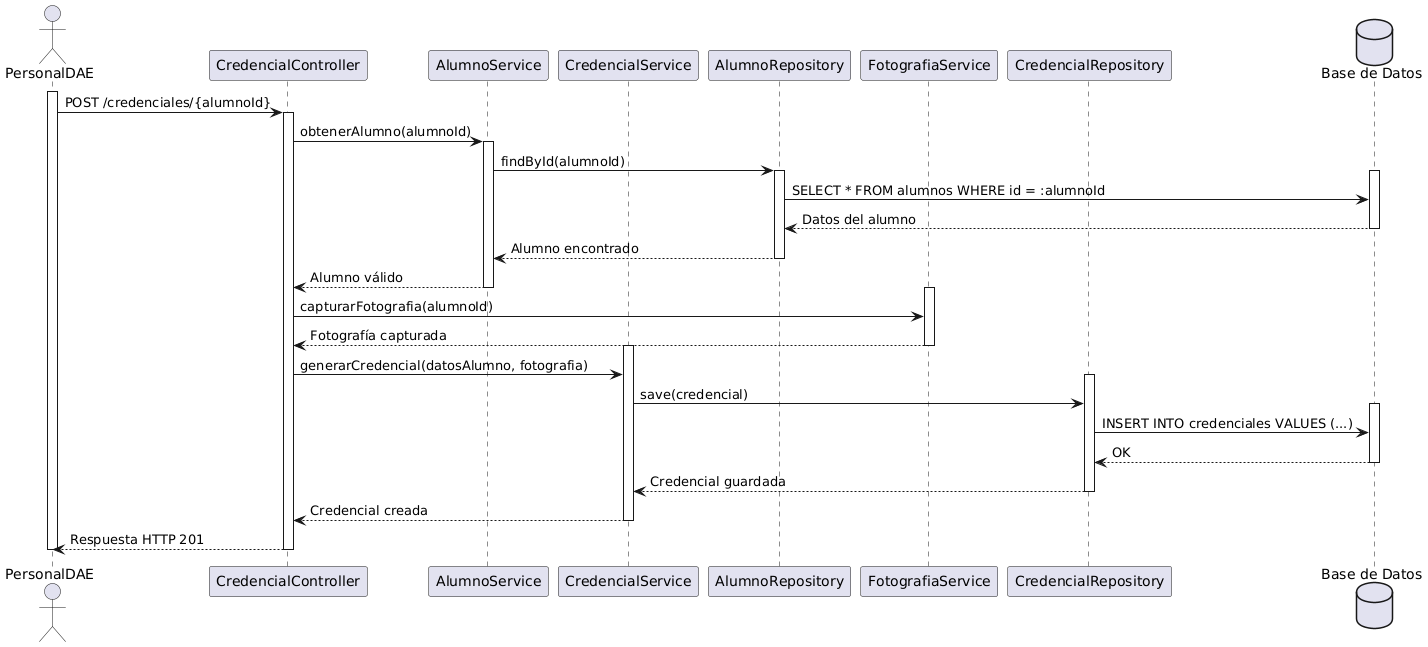
\includegraphics[width=1\textwidth]{Secuencia/CU-22_23.png}}
		\caption{Diagrama de secuencia del caso de uso número 22 y 23 (Crear credencial y capturar fotografía estudiantil).}
		\label{fig:Diagrama de secuencia CU-22 y CU23}
	\end{center}
\end{figure}

En el diagrama de secuencia \ref{fig:Diagrama de secuencia CU-22 y CU23} y se describe el proceso planeado para el caso de uso \hyperlink{CU-22}{CU-22 Crear credencia} y \hyperlink{CU-23}{CU-23 Capturar fotografía estudiantil}, mostrando las interacciones que tendrá con la vista, el controlador, el servicio, el repositorio y la base de datos.

\newpage

\subsection{SE-23 Consultar lista de periodo de ETS}

\begin{figure}[htbp!]
	\begin{center}
		\fbox{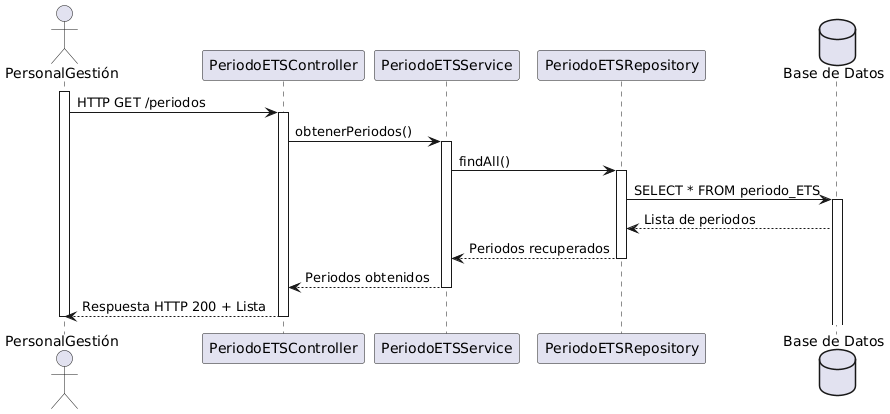
\includegraphics[width=1\textwidth]{Secuencia/CU-24.png}}
		\caption{Diagrama de secuencia del caso de uso número 24 (Consultar lista de periodo de ETS).}
		\label{fig:Diagrama de secuencia CU-24}
	\end{center}
\end{figure}

En el diagrama de secuencia \ref{fig:Diagrama de secuencia CU-24} se describe el proceso planeado para el caso de uso \hyperlink{CU-24}{CU-24 Consultar lista de periodo de ETS}, mostrando las interacciones que tendrá con la vista, el controlador, el servicio, el repositorio y la base de datos.

\newpage

\subsection{SE-24 Dar de alta de periodo de ETS}

\begin{figure}[htbp!]
	\begin{center}
		\fbox{\includegraphics[width=1\textwidth]{Secuencia/CU-25.png}}
		\caption{Diagrama de secuencia del caso de uso número 25 (Dar de alta de periodo de ETS).}
		\label{fig:Diagrama de secuencia CU-25}
	\end{center}
\end{figure}

En el diagrama de secuencia \ref{fig:Diagrama de secuencia CU-25} se describe el proceso planeado para el caso de uso \hyperlink{CU-25}{CU-25 Dar de alta de periodo de ETS}, mostrando las interacciones que tendrá con la vista, el controlador, el servicio, el repositorio y la base de datos.

\newpage

\subsection{SE-25 Consultar lista de ETS}

\begin{figure}[htbp!]
	\begin{center}
		\fbox{\includegraphics[width=1\textwidth]{Secuencia/CU-28.png}}
		\caption{Diagrama de secuencia del caso de uso número 28 (Consultar lista de ETS).}
		\label{fig:Diagrama de secuencia CU-28}
	\end{center}
\end{figure}

En el diagrama de secuencia \ref{fig:Diagrama de secuencia CU-28} se describe el proceso planeado para el caso de uso \hyperlink{CU-28}{CU-28 Consultar lista de ETS}, mostrando las interacciones que tendrá con la vista, el controlador, el servicio, el repositorio y la base de datos.

\newpage

\subsection{SE-26 Dar de alta ETS}

\begin{figure}[htbp!]
	\begin{center}
		\fbox{\includegraphics[width=1\textwidth]{Secuencia/CU-29.png}}
		\caption{Diagrama de secuencia del caso de uso número 29 (Dar de alta ETS).}
		\label{fig:Diagrama de secuencia CU-29}
	\end{center}
\end{figure}

En el diagrama de secuencia \ref{fig:Diagrama de secuencia CU-29} se describe el proceso planeado para el caso de uso \hyperlink{CU-29}{CU-29 Dar de alta ETS}, mostrando las interacciones que tendrá con la vista, el controlador, el servicio, el repositorio y la base de datos.

\newpage

\subsection{SE-27 Consultar lista de personal de seguridad}

\begin{figure}[htbp!]
	\begin{center}
		\fbox{\includegraphics[width=1\textwidth]{Secuencia/CU-32.png}}
		\caption{Diagrama de secuencia del caso de uso número 32 (Consultar lista de personal de seguridad).}
		\label{fig:Diagrama de secuencia CU-32}
	\end{center}
\end{figure}

En el diagrama de secuencia \ref{fig:Diagrama de secuencia CU-32} se describe el proceso planeado para el caso de uso \hyperlink{CU-32}{CU-32 Consultar lista de personal de seguridad}, mostrando las interacciones que tendrá con la vista, el controlador, el servicio, el repositorio y la base de datos.

\newpage

\subsection{SE-28 Dar de alta personal de seguridad}

\begin{figure}[htbp!]
	\begin{center}
		\fbox{\includegraphics[width=1\textwidth]{Secuencia/CU-33.png}}
		\caption{Diagrama de secuencia del caso de uso número 33 (Dar de alta personal de seguridad).}
		\label{fig:Diagrama de secuencia CU-33}
	\end{center}
\end{figure}

En el diagrama de secuencia \ref{fig:Diagrama de secuencia CU-33} se describe el proceso planeado para el caso de uso \hyperlink{CU-33}{CU-33 Dar de alta personal de seguridad}, mostrando las interacciones que tendrá con la vista, el controlador, el servicio, el repositorio y la base de datos.

\newpage

\subsection{SE-29 Consultar lista de docentes}

\begin{figure}[htbp!]
	\begin{center}
		\fbox{\includegraphics[width=1\textwidth]{Secuencia/CU-36.png}}
		\caption{Diagrama de secuencia del caso de uso número 36 (Consultar lista de docentes).}
		\label{fig:Diagrama de secuencia CU-36}
	\end{center}
\end{figure}

En el diagrama de secuencia \ref{fig:Diagrama de secuencia CU-36} se describe el proceso planeado para el caso de uso \hyperlink{CU-36}{CU-36 Consultar lista de docentes}, mostrando las interacciones que tendrá con la vista, el controlador, el servicio, el repositorio y la base de datos.

\newpage

\subsection{SE-30 Dar de alta docente}

\begin{figure}[htbp!]
	\begin{center}
		\fbox{\includegraphics[width=1\textwidth]{Secuencia/CU-37.png}}
		\caption{Diagrama de secuencia del caso de uso número 37 (Dar de alta docente).}
		\label{fig:Diagrama de secuencia CU-37}
	\end{center}
\end{figure}

En el diagrama de secuencia \ref{fig:Diagrama de secuencia CU-37} se describe el proceso planeado para el caso de uso \hyperlink{CU-37}{CU-37 Dar de alta docente}, mostrando las interacciones que tendrá con la vista, el controlador, el servicio, el repositorio y la base de datos.

\newpage

\subsection{SE-31 Solicitar desbloqueo de cuenta}

\begin{figure}[htbp!]
	\begin{center}
		\fbox{\includegraphics[width=1\textwidth]{Secuencia/CU-40.png}}
		\caption{Diagrama de secuencia del caso de uso número 40 (Solicitar desbloqueo de cuenta).}
		\label{fig:Diagrama de secuencia CU-40}
	\end{center}
\end{figure}

En el diagrama de secuencia \ref{fig:Diagrama de secuencia CU-40} se describe el proceso planeado para el caso de uso \hyperlink{CU-40}{CU-40 Solicitar desbloqueo de cuenta}, mostrando las interacciones que tendrá con la vista, el controlador, el servicio, el repositorio y la base de datos.

\newpage

\subsection{SE-32 Iniciar sesión del sistema web}

\begin{figure}[htbp!]
	\begin{center}
		\fbox{\includegraphics[width=1\textwidth]{Secuencia/CU-41.png}}
		\caption{Diagrama de secuencia del caso de uso número 41 (Iniciar sesión del sistema web).}
		\label{fig:Diagrama de secuencia CU-41}
	\end{center}
\end{figure}


En el diagrama de secuencia \ref{fig:Diagrama de secuencia CU-41} se describe el proceso planeado para el caso de uso \hyperlink{CU-41}{CU-41 Iniciar sesión del sistema web}, mostrando las interacciones que tendrá con la vista, el controlador, el servicio, el repositorio y la base de datos.

\newpage

\subsection{SE-33 Asignar docente de remplazo}

\begin{figure}[htbp!]
	\begin{center}
		\fbox{\includegraphics[width=1\textwidth]{Secuencia/CU-42.png}}
		\caption{Diagrama de secuencia del caso de uso número 42 (Asignar docente de remplazo).}
		\label{fig:Diagrama de secuencia CU-42}
	\end{center}
\end{figure}

En el diagrama de secuencia \ref{fig:Diagrama de secuencia CU-42} se describe el proceso planeado para el caso de uso \hyperlink{CU-42}{CU-42 Asignar docente de remplazo}, mostrando las interacciones que tendrá con la vista, el controlador, el servicio, el repositorio y la base de datos.